% Dieses Dokument muss mit PDFLatex gesetzt werden
% Vorteil: Grafiken koennen als jpg, png, ... verwendet werden
%          und die Links im Dokument sind auch gleich richtig
%
%Ermöglicht \\ bei der Titelseite (z.B. bei supervisor)
%Siehe https://github.com/latextemplates/uni-stuttgart-cs-cover/issues/4
\RequirePackage{kvoptions-patch}

%English:
\let\ifdeutsch\iffalse
\let\ifenglisch\iftrue

%German:
%\let\ifdeutsch\iftrue
%\let\ifenglisch\iffalse

%
\ifenglisch
	\PassOptionsToClass{numbers=noenddot}{scrbook}
\else
	%()Aus scrguide.pdf - der Dokumentation von KOMA-Script)
	%Nach DUDEN steht in Gliederungen, in denen ausschließlich arabische Ziffern für die Nummerierung
	%verwendet werden, am Ende der Gliederungsnummern kein abschließender Punkt
	%(siehe [DUD96, R3]). Wird hingegen innerhalb der Gliederung auch mit römischen Zahlen
	%oder Groß- oder Kleinbuchstaben gearbeitet, so steht am Ende aller Gliederungsnummern ein
	%abschließender Punkt (siehe [DUD96, R4])
	\PassOptionsToClass{numbers=autoendperiod}{scrbook}
\fi

%Warns about outdated packages and missing caption delcarations
%See https://www.ctan.org/pkg/nag
\RequirePackage[l2tabu, orthodox]{nag}

%Neue deutsche Trennmuster
%Siehe http://www.ctan.org/pkg/dehyph-exptl und http://projekte.dante.de/Trennmuster/WebHome
%Nur für pdflatex, nicht für lualatex
\RequirePackage{ifluatex}
\ifluatex
%do not load anything
\else
	\ifdeutsch
		\RequirePackage[ngerman=ngerman-x-latest]{hyphsubst}
	\fi
\fi

\documentclass[
               fontsize=12pt, %Default: 11pt, bei Linux Libertine zu klein zum Lesen
% BEGINN: Optionen für typearea
               % paper=a4, CUSTOM OFF
               oneside,  % fuer die Betrachtung am Schirm ungeschickt
               BCOR=3mm, % Bindekorrektur
               DIV=12,   % je höher der DIV-Wert, desto mehr geht auf eine Seite. Gute werde sind zwischen DIV=12 und DIV=15
               % headinclude=true, CUSTOM OFF
               % footinclude=false, CUSTOM OFF
% ENDE: Optionen für typearea
%               titlepage,
               bibliography=totoc,
%               idxtotoc,   %Index ins Inhaltsverzeichnis
%                liststotoc, %List of X ins Inhaltsverzeichnis, mit liststotocnumbered werden die Abbildungsverzeichnisse nummeriert
               headsepline,
               cleardoublepage=empty,
               parskip=half,
%               draft    % um zu sehen, wo noch nachgebessert werden muss - wichtig, da Bindungskorrektur mit drin
               final   % ACHTUNG! - in pagestyle.tex noch Seitenstil anpassen
               ]{scrbook}


%%%
% Beschreibung:
% In dieser Datei werden zuerst die benoetigten Pakete eingebunden und
% danach diverse Optionen gesetzt. Achtung Reihenfolge ist entscheidend!
%
%%%


%%%
% Styleguide:
%
% Ein sehr kleiner Styleguide. Packages werden in Blöcken organisiert.
% Ein Block beginnt mit drei % in einer Zeile, dann % <Blocküberschrift>, dann
% eine Liste der möglichen Optionen und deren Einstellungen, Gründe und Kommentare
% eine % Zeile in der sonst nichts steht und dann wieder %%% in einer Zeile.
%
% Zwischen zwei Blöcken sind 2 Leerzeilen!
% Zu jedem Paket werden soviele Optionen wie möglich/nötig angegeben
%
%%%

%%%
% Codierung
% Wir sind im 21 Jahrhundert, utf-8 löst so viele Probleme.
%
% Mit UTF-8 funktionieren folgende Pakete nicht mehr. Bitte beachten!
%   * fancyvrb mit §
%   * easylist -> http://www.ctan.org/tex-archive/macros/latex/contrib/easylist/
\ifluatex
%no package loading required
\else
\usepackage[utf8]{inputenc}
\fi
%
%%%

%%%
%Parallelbetrieb tex4ht und pdflatex
\makeatletter
\@ifpackageloaded{tex4ht}{\def\iftex4ht{\iftrue}}
                         {\def\iftex4ht{\iffalse}}
\makeatother
%%%


%%%
%Farbdefinitionen
\usepackage[hyperref,dvipsnames]{xcolor}
%

%%%
% Required for custom acronyms/glossaries style
% Left aligned Columns in tables with fixed width
% see http://tex.stackexchange.com/questions/91566/syntax-similar-to-centering-for-right-and-left
\usepackage{ragged2e}
%%%

%%%
% Abkürzungsverzeichnis
\usepackage{scrwfile} % Wichtig, ansonsten erscheint "No room for a new \write"
% siehe http://www.dickimaw-books.com/cgi-bin/faq.cgi?action=view&categorylabel=glossaries#glsnewwriteexceeded
\usepackage[acronym,indexonlyfirst,nomain]{glossaries}
\ifdeutsch
\renewcommand*{\acronymname}{Abkürzungsverzeichnis}
\else
\renewcommand*{\acronymname}{List of Abbreviations}
\fi
\renewcommand*{\glsgroupskip}{}
%
% Removed Glossarie as a table as a quick fix to get the template working again
% see http://tex.stackexchange.com/questions/145579/how-to-print-acronyms-of-glossaries-into-a-table
%
\makenoidxglossaries
%%%


%%%
% Neue deutsche Rechtschreibung und Literatur statt "Literature", Nachfolger von ngerman.sty
\ifdeutsch
% letzte Sprache ist default, Einbindung von "american" ermöglicht \begin{otherlanguage}{amercian}...\end{otherlanguage} oder \foreignlanguage{american}{Text in American}
% see also http://tex.stackexchange.com/a/50638/9075
\usepackage[american,ngerman]{babel}
% Ein "abstract" ist eine "Kurzfassung", keine "Zusammenfassung"
\addto\captionsngerman{%
	\renewcommand\abstractname{Kurzfassung}%
}
\else
%
%
% if you are writing in english
% last language is the default language
\usepackage[ngerman,american]{babel}
\fi
%
%%%

%%%
% Anführungszeichen
% Zitate in \enquote{...} setzen, dann werden automatisch die richtigen Anführungszeichen verwendet.
\usepackage{csquotes}
%%%


%%%
% erweitertes Enumerate
\usepackage{paralist}
%
%%%


%%%
% fancyheadings (nicht nur) fuer koma
\usepackage[automark]{scrlayer-scrpage}
%
%%%


%%%
%Mathematik
%
\usepackage[]{amsmath} % Viele Mathematik-Sachen: Doku: /usr/share/doc/texmf/latex/amsmath/amsldoc.dvi.gz
\PassOptionsToPackage{fleqn,leqno}{amsmath} % options must be passed this way, otherwise it does not work with glossaries
%fleqn (=Gleichungen linksbündig platzieren) funktioniert nicht direkt. Es muss noch ein Patch gemacht werden:
%\addtolength\mathindent{1em}%work-around ams-math problem with align and 9 -> 10. Does not work with glossaries, No visual changes.
\usepackage{mathtools} %fixes bugs in AMS math
%
%for theorems, replacement for amsthm
\usepackage[amsmath,hyperref]{ntheorem}
\theorempreskipamount 2ex plus1ex minus0.5ex
\theorempostskipamount 2ex plus1ex minus0.5ex
\theoremstyle{break}
\newtheorem{definition}{Definition}[section]
%
%%%


%%%
% Intelligentes Leerzeichen um hinter Abkürzungen die richtigen Abstände zu erhalten, auch leere.
% siehe commands.tex \gq{}
\usepackage{xspace}
%Macht \xspace und \enquote kompatibel
\makeatletter
\xspaceaddexceptions{\grqq \grq \csq@qclose@i \} }
\makeatother
%
%%%


%%%
% Anhang
\usepackage{appendix}
%[toc,page,title,header]
%
%%%


%%%
% Grafikeinbindungen
\usepackage{graphicx}%Parameter "pdftex" unnoetig
\graphicspath{{\getgraphicspath}}
\newcommand{\getgraphicspath}{graphics/}
%
%%%


%%%
% Enables inclusion of SVG graphics - 1:1 approach
% This is NOT the approach of http://www.ctan.org/tex-archive/info/svg-inkscape,
% which allows text in SVG to be typeset using LaTeX
% We just include the SVG as is
\usepackage{epstopdf}
\epstopdfDeclareGraphicsRule{.svg}{pdf}{.pdf}{%
  inkscape -z -D --file=#1 --export-pdf=\OutputFile
}
%
%%%


%%%
% Enables inclusion of SVG graphics - text-rendered-with-LaTeX-approach
% This is the approach of http://www.ctan.org/tex-archive/info/svg-inkscape,
\newcommand{\executeiffilenewer}[3]{%
\IfFileExists{#2}
{
%\message{file #2 exists}
\ifnum\pdfstrcmp{\pdffilemoddate{#1}}%
{\pdffilemoddate{#2}}>0%
{\immediate\write18{#3}}
\else
{%\message{file up to date #2}
}
\fi%
}{
%\message{file #2 doesn't exist}
%\message{argument: #3}
%\immediate\write18{echo "test" > xoutput.txt}
\immediate\write18{#3}
}
}
\newcommand{\includesvg}[1]{%
\executeiffilenewer{#1.svg}{#1.pdf}%
{
inkscape -z -D --file=\getgraphicspath#1.svg %
--export-pdf=\getgraphicspath#1.pdf --export-latex}%
\input{\getgraphicspath#1.pdf_tex}%
}


%%%
\usepackage{siunitx}
%%%

%%%
% Tabellenerweiterungen
\usepackage{array} %increases tex's buffer size and enables ``>'' in tablespecs
\usepackage{longtable}
\usepackage{dcolumn} %Aligning numbers by decimal points in table columns
\ifdeutsch
	\newcolumntype{d}[1]{D{.}{,}{#1}}
\else
	\newcolumntype{d}[1]{D{.}{.}{#1}}
\fi

%
%%%

%%%
% Eine Zelle, die sich über mehrere Zeilen erstreckt.
% Siehe Beispieltabelle in Kapitel 2
\usepackage{multirow}
%
%%%

%%%
%Fuer Tabellen mit Variablen Spaltenbreiten
%\usepackage{tabularx}
%\usepackage{tabulary}
%
%%%


%%%
% Links verhalten sich so, wie sie sollen
\usepackage{url}
%
%Use text font as url font, not the monospaced one
%see comments at http://tex.stackexchange.com/q/98463/9075
\urlstyle{same}
%
%Hint by http://tex.stackexchange.com/a/10419/9075
\makeatletter
\g@addto@macro{\UrlBreaks}{\UrlOrds}
\makeatother
%
%%%


%%%
% Index über Begriffe, Abkürzungen
%\usepackage{makeidx} makeidx ist out -> http://xindy.sf.net verwenden
%
%%%

%%%
%lustiger Hack fuer das Abkuerzungsverzeichnis
%nach latex durchlauf folgendes ausfuehren
%makeindex main.nlo -s nomencl.ist -o main.nls
%danach nochmal latex
%\usepackage{nomencl}
%    \let\abk\nomenclature %Deutsche Ueberschrift setzen
%          \renewcommand{\nomname}{List of Abbreviations}
%        %Punkte zw. Abkuerzung und Erklaerung
%          \setlength{\nomlabelwidth}{.2\hsize}
%          \renewcommand{\nomlabel}[1]{#1 \dotfill}
%        %Zeilenabstaende verkleinern
%          \setlength{\nomitemsep}{-\parsep}
%    \makenomenclature
%
%%%

%%%
% Logik für Tex
\usepackage{ifthen} %fuer if-then-else @ commands.tex
%
%%%


%%%
%
\usepackage{listings}
%
%%%


%%%
%Alternative zu Listings ist fancyvrb. Kann auch beides gleichzeitig benutzt werden.
\usepackage{fancyvrb}
%\fvset{fontsize=\small} %Groesse fuer den Fliesstext. Falls deaktiviert: \normalsize
%Funktioniert mit UTF-8 nicht mehr
%\DefineShortVerb{\§} %Somit kann im Text ganz einfach |verbatim| text gesetzt werden.
\RecustomVerbatimEnvironment{Verbatim}{Verbatim}{fontsize=\footnotesize}
\RecustomVerbatimCommand{\VerbatimInput}{VerbatimInput}{fontsize=\footnotesize}
%
%%%


%%%
% Bildunterschriften bei floats genauso formatieren wie bei Listings
% Anpassung wird unten bei den newfloat-Deklarationen vorgenommen
% https://www.ctan.org/pkg/caption2 is superseeded by this package.
\usepackage{caption}
%
%%%


%%%
% Ermoeglicht es, Abbildungen um 90 Grad zu drehen
% Alternatives Paket: rotating Allerdings wird hier nur das Bild gedreht, während bei lscape auch die PDF-Seite gedreht wird.
%Das Paket lscape dreht die Seite auch nicht
\usepackage{pdflscape}
%
%%%


%%%
% Fuer listings
% Wird für fancyvrb und für lstlistings verwendet
\usepackage{float}

%\usepackage{floatrow}
%% zustäzlich für den Paramter [H] = Floats WIRKLICH da wo sie deklariert wurden paltzieren - ganz ohne Kompromisse
% floatrow ist der Nachfolger von float
% Allerdings macht floatrow in manchen Konstellationen Probleme. Deshalb ist das Paket deaktiviert.
%
%%%



%%%
% Fuer Abbildungen innerhalb von Abbildungen
% Ersetzt das Paket subfigure
%
% Due to bug #24 in the caption package we need to update caption3.sty at the moment manualy to use subfig.
% Bug #24: http://sourceforge.net/p/latex-caption/tickets/24/
% corrected caption3.sty: http://sourceforge.net/p/latex-caption/code/HEAD/tree/branches/3.3/tex/caption3.sty
%
\usepackage[caption=false, lofdepth=1, lotdepth, margin=5pt]{subfig}
%
%%%




%%%
% Fußnoten
%
%\usepackage{dblfnote}  %Zweispaltige Fußnoten
%
% Keine hochgestellten Ziffern in der Fußnote (KOMA-Script-spezifisch):
%\deffootnote[1.5em]{0pt}{1em}{\makebox[1.5em][l]{\bfseries\thefootnotemark}}
%
% Abstand zwischen Fußnoten vergrößern:
%\setlength{\footnotesep}{.85\baselineskip}
%
%
%
%Folgendes Kommando deaktiviert die Trennlinie zur Fußnote
%\renewcommand{\footnoterule}{}
%
\addtolength{\skip\footins}{\baselineskip} % Abstand Text <-> Fußnote
%
% Fußnoten immer ganz unten auf einer \raggedbottom-Seite
% fnpos kommt aus dem yafoot package
\usepackage{fnpos}
\makeFNbelow
\makeFNbottom
%
%%%


%%%
%
\raggedbottom     % Variable Seitenhöhen zulassen
%
%%%


%%%
% Falls die Seitenzahl bei einer Referenz auf eine Abbildung nur dann angegeben werden soll,
% falls sich die Abbildung nicht auf der selben Seite befindet...
\iftex4ht
%tex4ht does not work well with vref, therefore we emulate vref behavior
\newcommand{\vref}[1]{\ref{#1}}
\else
\ifdeutsch
\usepackage[ngerman]{varioref}
\else
\usepackage{varioref}
\fi
\fi
%%%

%%%
% Noch schoenere Tabellen als mit booktabs mit http://www.zvisionwelt.de/downloads.html
\usepackage{booktabs}
%
%\usepackage[section]{placeins}
%
%%%


%%%
%Fuer Graphiken. Allerdings funktioniert es nicht zusammen mit pdflatex
%\usepackage{gastex} % \tolarance kann dann nicht mehr umdefiniert werden
%
%%%


%%%
%
%\usepackage{multicol}
%\usepackage{setspace} % kollidiert mit diplomarbeit.sty
%
%http://www.tex.ac.uk/cgi-bin/texfaq2html?label=floats
%\usepackage{flafter} %floats IMMER nach ihrer Deklaration platzieren
%
%%%


%%%
%schoene TODOs
\usepackage{todonotes}
\let\xtodo\todo
\renewcommand{\todo}[1]{\xtodo[inline,color=black!5]{#1}}
\newcommand{\utodo}[1]{\xtodo[inline,color=green!5]{#1}}
\newcommand{\itodo}[1]{\xtodo[inline]{#1}}
%
%%%


%%%
%biblatex statt bibtex
\usepackage[
  backend       = biber, %biber does not work with 64x versions alternative: bibtex8
						 %minalphanames only works with biber backend
  sortcites     = true,
  bibstyle      = alphabetic,
  citestyle     = alphabetic,
  firstinits    = true,
  useprefix     = true, %"von, van, etc." will be printed, too. See below.
  minnames      = 1,
  minalphanames = 3,
  maxalphanames = 4,
  maxbibnames   = 99,
  maxcitenames  = 3,
  natbib        = true,
  eprint        = true,
  url           = true,
  doi           = true,
  isbn          = false,
  backref       = true]{biblatex}
\bibliography{bibliography}
%\addbibresource[datatype=bibtex]{bibliography.bib}

%Do not put "vd" in the label, but put it at "\citeauthor"
%Source: http://tex.stackexchange.com/a/30277/9075
\makeatletter
\AtBeginDocument{\toggletrue{blx@useprefix}}
\AtBeginBibliography{\togglefalse{blx@useprefix}}
\makeatother

%Thin spaces between initials
%http://tex.stackexchange.com/a/11083/9075
\renewrobustcmd*{\bibinitdelim}{\,}

%Keep first and last name together in the bibliography
%http://tex.stackexchange.com/a/196192/9075
\renewcommand*\bibnamedelimc{\addnbspace}
\renewcommand*\bibnamedelimd{\addnbspace}

%Replace last "and" by comma in bibliography
%See http://tex.stackexchange.com/a/41532/9075
\AtBeginBibliography{%
  \renewcommand*{\finalnamedelim}{\addcomma\space}%
}

\DefineBibliographyStrings{ngerman}{
  backrefpage  = {zitiert auf S\adddot},
  backrefpages = {zitiert auf S\adddot},
  andothers    = {et\ \addabbrvspace al\adddot},
  %Tipp von http://www.mrunix.de/forums/showthread.php?64665-biblatex-Kann-%DCberschrift-vom-Inhaltsverzeichnis-nicht-%E4ndern&p=293656&viewfull=1#post293656
  bibliography = {Literaturverzeichnis}
}

%enable hyperlinked author names when using \citeauthor
%source: http://tex.stackexchange.com/a/75916/9075
\DeclareCiteCommand{\citeauthor}
  {\boolfalse{citetracker}%
   \boolfalse{pagetracker}%
   \usebibmacro{prenote}}
  {\ifciteindex
     {\indexnames{labelname}}
     {}%
   \printtext[bibhyperref]{\printnames{labelname}}}
  {\multicitedelim}
  {\usebibmacro{postnote}}

%natbib compatibility
%\newcommand{\citep}[1]{\cite{#1}}
%\newcommand{\citet}[1]{\citeauthor{#1} \cite{#1}}
%Beginning of sentence - analogous to cleveref - important for names such as "zur Muehlen"
%\newcommand{\Citep}[1]{\cite{#1}}
%\newcommand{\Citet}[1]{\Citeauthor{#1} \cite{#1}}
%%%


%%%
% Blindtext. Paket "blindtext" ist fortgeschritterner als "lipsum" und kann auch Mathematik im Text (http://texblog.org/2011/02/26/generating-dummy-textblindtext-with-latex-for-testing/)
% kantlipsum (https://www.ctan.org/tex-archive/macros/latex/contrib/kantlipsum) ist auch ganz nett, aber eben auch keine Mathematik
% Wird verwendet, um etwas Text zu erzeugen, um eine volle Seite wegen Layout zu sehen.
\usepackage[math]{blindtext}
%%%

%%%
% Neue Pakete bitte VOR hyperref einbinden. Insbesondere bei Verwendung des
% Pakets "index" wichtig, da sonst die Referenzierung nicht funktioniert.
% Für die Indizierung selbst ist unter http://xindy.sourceforge.net
% ein gutes Tool zu erhalten
%%%


%%%
%
% hier also neue packages einbinden
%
%%%


%%%
% ggf.in der Endversion komplett rausnehmen. dann auch \href in commands.tex aktivieren
% Alle Optionen nach \hypersetup verschoben, sonst crash
%
\usepackage[]{hyperref}%siehe auch: "Praktisches LaTeX" - www.itp.uni-hannover.de/~kreutzm
%
%% Da es mit KOMA 3 und xcolor zu Problemen mit den global Options kommt MÜSSEN die Optionen so gesetzt werden.
%

% Eigene Farbdefinitionen ohne die Namen des xcolor packages
\definecolor{darkblue}{rgb}{0,0,.5}
\definecolor{black}{rgb}{0,0,0}

\hypersetup{
    breaklinks=true,
    bookmarksnumbered=true,
    bookmarksopen=true,
    bookmarksopenlevel=1,
    breaklinks=true,
    colorlinks=true,
    pdfstartview=Fit,
    pdfpagelayout=TwoPageRight, % zweiseitige Darstellung: ungerade Seiten rechts im PDF-Viewer - siehe auch http://tex.stackexchange.com/a/21109/9075
    filecolor=darkblue,
    urlcolor=darkblue,
    linkcolor=black,
    citecolor=black
}
%
%%%


%%%
% cleveref für cref statt autoref, da cleveref auch bei Definitionen funktioniert
\ifdeutsch
\usepackage[ngerman,capitalise,nameinlink,noabbrev]{cleveref}
\else
\usepackage[capitalise,nameinlink,noabbrev]{cleveref}
\fi
%%%


%%%
% Zur Darstellung von Algorithmen
% Algorithm muss nach hyperref geladen werden
\usepackage[chapter]{algorithm}
\usepackage[]{algpseudocode}
%
%%%


%%%
% Schriften
%%%
%
\automark[section]{chapter}
\ifenglisch
%serif font also in heading, foot and page number (contained in foot)
\setkomafont{pageheadfoot}{\normalfont\rmfamily}
\setkomafont{pagenumber}{\normalfont\rmfamily}
\else
%sans serif font in German texts
\setkomafont{pageheadfoot}{\normalfont\sffamily}
\setkomafont{pagenumber}{\normalfont\sffamily}
\fi
%
%\setheadsepline[.4pt]{.4pt} %funktioniert nicht: Alle Linien sind hier weg
%
%%%

%%%
%
\ifenglisch
% Fuer englische Texte sind serifenhafte Ueberschriften gut. Deshalb hier der Befehl zum Aktivieren von serifenhaften Ueberschriften
\setkomafont{disposition}{\normalfont\rmfamily}

% Bei englischen Texten das Label (optionaler Eintrag bei \item) bei description-Umgegungen nur auf fett und nicht fett+serifenlos stellen.
\setkomafont{descriptionlabel}{\normalfont\bfseries}
\fi
%
%%%

%%%
% Fuer deutsche Texte: Weniger Silbentrennung, mehr Abstand zwischen den Woertern
\ifdeutsch
\setlength{\emergencystretch}{3em} % Silbentrennung reduzieren durch mehr frei Raum zwischen den Worten
\fi
%%%

%Symbole
%--------
%\usepackage[geometry]{ifsym} % \BigSquare
%\usepackage{mathabx}
%\usepackage{stmaryrd} %fuer \ovee, \owedge, \otimes
%\usepackage{marvosym} %fuer \Writinghand %patched to not redefine \Rightarrow
%\usepackage{mathrsfs} %mittels \mathscr{} schoenen geschwungenen Buchstaben erzeugen
%\usepackage{calrsfs} %\mathcal{} ein bisserl dickeren buchstaben erzeugen - sieht net so gut aus.
                      %durch mathpazo ist das schon definiert
\usepackage{amssymb}

%For \texttrademark{}
\usepackage{textcomp}

%name-clashes von marvosym und mathabx vermeiden:
\def\delsym#1{%
%  \expandafter\let\expandafter\origsym\expandafter=\csname#1\endcsname
%  \expandafter\let\csname orig#1\endcsname=\origsym
  \expandafter\let\csname#1\endcsname=\relax
}

%\usepackage{pifont}
%\usepackage{bbding}
%\delsym{Asterisk}
%\delsym{Sun}\delsym{Mercury}\delsym{Venus}\delsym{Earth}\delsym{Mars}
%\delsym{Jupiter}\delsym{Saturn}\delsym{Uranus}\delsym{Neptune}
%\delsym{Pluto}\delsym{Aries}\delsym{Taurus}\delsym{Gemini}
%\delsym{Rightarrow}
%\usepackage{mathabx} - Ueberschreibt leider zu viel - und die \le-Zeichen usw. sehen nicht gut aus!

%Fallback-Schriftart
\usepackage{lmodern}  % Latin Modern Fonts sind die Nachfolger von Computer Modern, den LaTeX-Standardfonts
%Quelle: http://homepage.ruhr-uni-bochum.de/Georg.Verweyen/pakete.html
%Allerdings sieht diese Schritart in Diplomarbeiten fuer Fliesstext auch nicht besonders schoen aus.
%Trotzdem ist sie fuer Programmcode gut geeignet

%Schriftart fuer die Ueberschriften - ueberschreibt lmodern
\usepackage[scaled=.95]{helvet}

% Für Schreibschrift würde tun, muss aber ned
%\usepackage{mathrsfs} %  \mathscr{ABC}

%Schriftart fuer den Fliesstext - ueberschreibt lmodern
%
\ifdeutsch
%
%Linux Libertine, siehe http://www.linuxlibertine.org/
%Packageparamter [osf] = Minuskel-Ziffern
%rm = libertine im Brottext, Linux Biolinum NICHT als serifenlose Schrift, sondern helvet (von oben) beibehalten
\usepackage[rm]{libertine}
%
%Alternative Schriftart: Palantino, Packageparamter [osf] = Minuskel-Ziffern
%\usepackage{mathpazo} %ftp://ftp.dante.de/tex-archive/fonts/mathpazo/ - Tipp aus DE-TEX-FAQ 8.2.1
%
\fi

\ifenglisch
%
\usepackage{charter} %Charter fuer englische Texte
\linespread{1.4} % Durchschuss für Charter leicht erhöhen
%
%\usepackage{mathptmx} %Times fuer englische Texte. Sieht nicht sooo gut aus.
%
%Fallback ist lmodern, die oben eingebunden wurde
\fi

%Schriftart fuer Programmcode - ueberschreibt lmodern
%Falls auskommentiert, wird die Standardschriftart lmodern genommen
%\usepackage[scaled=.92]{luximono} % Fuer schreibmaschinenartige Schluesselwoerter in den Listings - geht bei alten Installationen nicht, da einige Fontshapes (<>=) fehlen
%\usepackage{courier}
\usepackage[scaled=0.83]{beramono} %BeraMono als Typewriter-Schrift, Tipp von http://tex.stackexchange.com/a/71346/9075

\ifluatex
\else
\usepackage[T1]{fontenc}
\fi


% optischer Randausgleich - bei miktex gleich dabei - bei linux von
%  http://www.ctan.org/tex-archive/macros/latex/contrib/microtype/
%  herunterladen 
\usepackage{microtype}
%Falls bei einer Silbentrennung ploetzlich eine ganze Zeile fehlt (passiert unter Windows XP mit MikTex 2.5 und foxit reader als pdfreader
%\usepackage{pdfcprot}
%ausprobieren. Dieses erzeugt allerdings nur für Palatino (in dieser Vorlage die Default-Schrift) einen guten optischen Randausgleich
%Falls alle Stricke reissen, muss leider auf den optischen Randausgleich verzichtet werden.

%fuer microtype
%tracking=true muss als Parameter des microtype-packages mitgegeben werden
%
%Deaktiviert, da dies bei Algorithmen seltsam aussieht
%
%\DeclareMicrotypeSet*[tracking]{my}{ font = */*/*/sc/* }% 
%\SetTracking{ encoding = *, shape = sc }{ 45 }% Hier wird festgelegt,
            % dass alle Passagen in Kapitälchen automatisch leicht
            % gesperrt werden.
			% Quelle: http://homepage.ruhr-uni-bochum.de/Georg.Verweyen/pakete.html

%
%%%


%%%
% Links auf Gleitumgebungen springen nicht zur Beschriftung,
% Doc: http://mirror.ctan.org/tex-archive/macros/latex/contrib/oberdiek/hypcap.pdf
% sondern zum Anfang der Gleitumgebung
\usepackage[all]{hypcap}
%%%


%%%
% Deckblattstyle
%
\ifdeutsch
	\PassOptionsToPackage{language=german}{uscs-cover}
\else
	\PassOptionsToPackage{language=english}{uscs-cover}
\fi

\usepackage[
    title={Developing a Distributed Media Streaming Application},
    author={Alexander Zarges, Nicolas Drebenstedt},
    type=master,
    course={Internationaler Studiengang\\ Medieninformatik},
    examiner={Prof.\ Dr.\ Gefei Zhang\\Prof.\ Dr.-Ing.\ Kai Uwe Barthel},
    startdate={October 25, 2018},
    enddate={March 18, 2019},
    ]{uscs-cover}
%
%%%


%%%
%Bugfixes packages
%\usepackage{fixltx2e} %Fuer neueste LaTeX-Installationen nicht mehr benoetigt - bereinigte einige Ungereimtheiten, die auf Grund von Rueckwaertskompatibilitaet beibahlten wurden.
%\usepackage{mparhack} %Fixt die Position von marginpars (die in DAs selten bis gar nicht gebraucht werden}
%\usepackage{ellipsis} %Fixt die Abstaende vor \ldots. Wird wohl auch nicht benoetigt.
%
%%%


%%%
% Rand
%Viele Moeglichkeiten, die Raender im Dokument einzustellen.
%Satzspiegel neu berechnen. Dokumentation dazu ist in "scrguide.pdf" von KOMA-Skript zu finden
%  Optionen werden bei \documentclass[] in main.tex mitgegeben.
\typearea[current]{current} %neu berechnen, da neue Schrift eingebunden

\usepackage{a4}
\usepackage{a4wide}
\areaset{170mm}{277mm} %a4:29,7hochx21mbreit

%Wer die Masse direkt eingeben moechte:
%Bei diesem Beispiel wird die Regel nicht beachtet, dass der innere Rand halb so gross wie der aussere Rand und der obere Rand halb so gross wie der untere Rand sein sollte
\usepackage[inner=4.0cm, outer=3.0cm, includefoot, top=3.0cm, bottom=1.5cm]{geometry}

%
%%%


%%%
% Optionen
%
\captionsetup{
  format=hang,
  labelfont=bf,
  justification=justified,
  %single line captions should be centered, multiline captions justified
  singlelinecheck=true
}
%
%neue float Umgebung fuer Listings, die mittels fancyvrb gesetzt werden sollen
\floatstyle{ruled}
\newfloat{Listing}{tbp}{code}[chapter]
\crefname{Listing}{Listing}{Listings}
\newfloat{Algorithmus}{tbp}{alg}[chapter]
\ifdeutsch
\crefname{Algorithmus}{Algorithmus}{Algorithmus}
\else
\crefname{Algorithmus}{Algorithm}{Algorithms}
\fi
%
%amsmath
%\numberwithin{equation}{section}
%\renewcommand{\theequation}{\thesection.\Roman{equation}}
%
%pdftex
\pdfcompresslevel=9
%
%Tabellen (array.sty)
\setlength{\extrarowheight}{1pt}
%
%
%%%

%%%
% unterschiedliche Chapter-Styles
% u.a. Paket fncychap
% Andere Kapitelueberschriften
% falls einem der Standard von KOMA nicht gefaellt...
% Falls man zurück zu KOMA moechte, dann muss jede der vier folgenden Moeglichkeiten deaktiviert sein.

% 1. Moeglichkeit
%\usepackage[Sonny]{fncychap}
%oder
%\usepackage[Bjarne]{fncychap}
%oder
%\usepackage[Lenny]{fncychap}

% 2. Moeglichkeit
\iffalse
\usepackage[Bjarne]{fncychap}
\ChNameVar{\Large\sf} \ChNumVar{\Huge} \ChTitleVar{\Large\sf}
\ChRuleWidth{0.5pt} \ChNameUpperCase
\fi

%Variante der 2. Moeglichkeit
\iffalse
\usepackage[Rejne]{fncychap}
\ChNameVar{\centering\Huge\rm\bfseries}
\ChNumVar{\Huge}
 \ChTitleVar{\centering\Huge\rm}
\ChNameUpperCase
\ChTitleUpperCase
\ChRuleWidth{1pt}
\fi

% 3. Moeglichkeit
\iffalse
\usepackage{fncychap}
\ChNameUpperCase
\ChTitleUpperCase
\ChNameVar{\raggedright\normalsize} %\rm
\ChNumVar{\bfseries\Large}
\ChTitleVar{\raggedright\Huge}
\ChRuleWidth{1pt}
\fi

% 4. Moeglichkeit
% Zur Aktivierierung "\iffalse" und "\fi" auskommentieren
% Innen drin kann man dann noch zwischen
%   * serifenloser Schriftart (eingestellt)
%   * serifenhafter Schriftart (wenn kein zusaetzliches Kommando aktiviert ist) und
%   * Kapitälchen wählen
\iffalse
\makeatletter
%\def\thickhrulefill{\leavevmode \leaders \hrule height 1ex \hfill \kern \z@}

%Fuer Kapitel mit Kapitelnummer
\def\@makechapterhead#1{%
  \vspace*{10\p@}%
  {\parindent \z@ \raggedright \reset@font
			%Default-Schrift: Serifenhaft (gut fuer englische Dokumente)
            %A) Fuer serifenlose Schrift:
            \fontfamily{phv}\selectfont
			%B) Fuer Kapitaelchen:
			%\fontseries{m}\fontshape{sc}\selectfont
            %C) Fuer ganz "normale" Schrift:
            %\normalfont 
			%
			\Large \@chapapp{} \thechapter
        \par\nobreak\vspace*{10\p@}%
        \interlinepenalty\@M
    {\Huge\bfseries\baselineskip3ex
	%Fuer Kapitaelchen folgende Zeile aktivieren:
	%\fontseries{m}\fontshape{sc}\selectfont
	#1\par\nobreak}
    \vspace*{10\p@}%
\makebox[\textwidth]{\hrulefill}%    \hrulefill alone does not work
    \par\nobreak
    \vskip 40\p@
  }}

  %Fuer Kapitel ohne Kapitelnummer (z.B. Inhaltsverzeichnis)
  \def\@makeschapterhead#1{%
  \vspace*{10\p@}%
  {\parindent \z@ \raggedright \reset@font
            \normalfont \vphantom{\@chapapp{} \thechapter}
        \par\nobreak\vspace*{10\p@}%
        \interlinepenalty\@M
    {\Huge \bfseries %
	%Default-Schrift: Serifenhaft (gut fuer englische Dokumente)
    %A) Fuer serifenlose Schrift folgende Zeile aktivieren:
    \fontfamily{phv}\selectfont
	%B) Fuer Kapitaelchen folgende Zeile aktivieren:
	%\fontseries{m}\fontshape{sc}\selectfont
	#1\par\nobreak}
    \vspace*{10\p@}%
\makebox[\textwidth]{\hrulefill}%    \hrulefill does not work
    \par\nobreak
    \vskip 40\p@
  }}
%
\makeatother
\fi

%%%

%%%
%Minitoc-Einstellungen
%\dominitoc
%\renewcommand{\mtctitle}{Inhaltsverzeichnis dieses Kapitels}
%
% Disable single lines at the start of a paragraph (Schusterjungen)
\clubpenalty = 10000
%
% Disable single lines at the end of a paragraph (Hurenkinder)
\widowpenalty = 10000 \displaywidowpenalty = 10000
%
%http://groups.google.de/group/de.comp.text.tex/browse_thread/thread/f97da71d90442816/f5da290593fd647e?lnk=st&q=tolerance+emergencystretch&rnum=5&hl=de#f5da290593fd647e
%Mehr Infos unter http://www.tex.ac.uk/cgi-bin/texfaq2html?label=overfull
\tolerance=2000
\setlength{\emergencystretch}{3pt}   % kann man evtl. auf 20 erhoehen
\setlength{\hfuzz}{1pt}
%
%%%


%%%
% Fuer listings.sty
\lstset{language=XML,
        showstringspaces=false,
        extendedchars=true,
        basicstyle=\footnotesize\ttfamily,
        commentstyle=\slshape,
        stringstyle=\ttfamily, %Original: \rmfamily, damit werden die Strings im Quellcode hervorgehoben. Zusaetzlich evtl.: \scshape oder \rmfamily durch \ttfamily ersetzen. Dann sieht's aus, wie bei fancyvrb
        breaklines=true,
        breakatwhitespace=true,
        columns=flexible,
        aboveskip=0mm, %deaktivieren, falls man lstlistings direkt als floating object benutzt (\begin{lstlisting}[float,...])
        belowskip=0mm, %deaktivieren, falls man lstlistings direkt als floating object benutzt (\begin{lstlisting}[float,...])
        captionpos=b
}
\ifdeutsch
\renewcommand{\lstlistlistingname}{Verzeichnis der Listings}
\fi
%
%%%


%%%
%fuer algorithm.sty: - falls Deutsch und nicht Englisch. Falls Englisch als Sprache gewählt wurde, bitte die folgenden beiden Zeilen auskommentieren.
\floatname{algorithm}{Algorithmus}
\ifdeutsch
\renewcommand{\listalgorithmname}{Verzeichnis der Algorithmen}
\fi
%
%%%


%%%
% Das Euro Zeichen
% Fuer Palatino (mathpazo.sty): richtiges Euro-Zeichen
% Alternative: \usepackage{eurosym}
\newcommand{\EUR}{\ppleuro}
%
%%%


%%%
%
% Float-placements - http://dcwww.camd.dtu.dk/~schiotz/comp/LatexTips/LatexTips.html#figplacement
% and http://people.cs.uu.nl/piet/floats/node1.html
\renewcommand{\topfraction}{0.85}
\renewcommand{\bottomfraction}{0.95}
\renewcommand{\textfraction}{0.1}
\renewcommand{\floatpagefraction}{0.75}
%\setcounter{totalnumber}{5}
%
%%%

%%%
%
% Bei Gleichungen nur dann die Nummer zeigen, wenn die Gleichung auch referenziert wird
%
% Funktioniert mit MiKTeX Stand 2012-01-13 nicht. Deshalb ist dieser Schalter deaktiviert.
%
%\mathtoolsset{showonlyrefs}
%
%%%


%%%
%ensure that floats covering a whole page are placed at the top of the page
%see http://tex.stackexchange.com/a/28565/9075
\makeatletter
\setlength{\@fptop}{0pt}
\setlength{\@fpbot}{0pt plus 1fil}
\makeatother
%%%


%%%
%Optischer Randausgleich
\usepackage{microtype}
%%%

%%%
%Package geometry to enlarge on page
%
%Source: http://www.howtotex.com/tips-tricks/change-margins-of-a-single-page/
%
%Normally, this should not be used as the typearea package calculates the margins perfectly
%\usepackage[
%  pass %just load the package and do not destory the work of typearea
%]{geometry}
%%%

%%%
% footnotes in tables
\usepackage{footnote}
\makesavenoteenv{tabular}
\makesavenoteenv{table}
% Reuse of footnotes
% Reuse of Footnotes, see http://tex.stackexchange.com/questions/10102/multiple-references-to-the-same-footnote-with-hyperref-support-is-there-a-bett
\crefformat{footnote}{#2\footnotemark[#1]#3}
%%%
\usepackage{titlesec}
\titleformat{\paragraph}
{\normalfont\normalsize}{\theparagraph}{1em}{}
\titlespacing*{\paragraph}
{0pt}{1.5ex plus 1ex minus .2ex}{0pt}

% quotes -> \say{}
\usepackage{dirtytalk}

\usepackage[utf8]{inputenc}

\usepackage{multicol}
\usepackage{courier}
\usepackage{listings} %For code in appendix
\lstset
{ %Formatting for code in appendix
    basicstyle=\footnotesize\ttfamily,
    numbers=left,
    stepnumber=1,
    showstringspaces=false,
    tabsize=1,
    breaklines=true,
    breakatwhitespace=false,
    xleftmargin=2em,
    escapechar=|
}

% tables
\usepackage{tabu}


%Der untere Rand darf "flattern"
\raggedbottom

%%%
% Wie tief wird das Inhaltsverzeichnis aufgeschlüsselt
% 0 --\chapter
% 1 --\section % fuer kuerzeres Inhaltsverzeichnis verwenden - oder minitoc benutzen
% 2 --\subsection
% 3 --\subsubsection
% 4 --\paragraph
\setcounter{tocdepth}{1}
%
%%%

\makeindex

%Angaben in die PDF-Infos uebernehmen
\makeatletter
\hypersetup{
            pdftitle={Developing a Distributed MediaStreaming Application},
            pdfauthor={Alexander Zarges, Nicolas Drebenstedt},
            pdfkeywords={},
            pdfsubject={}
}
\makeatother

\newacronym[plural={Application Programming Interfaces},shortplural={APIs}]{api}{API}{Application Programming Interface}
\newacronym{alm}{ALM}{Application Layer Multicast}
\newacronym{b2b}{B2B}{Business–to–Business}
\newacronym{bdi}{BDI}{Belief–Desire–Intention}
\newacronym{cbr}{CBR}{Constant Bitrate}
\newacronym{cli}{CLI}{Command–Line Interface}
\newacronym[plural={Content Delivery Networks},shortplural={CDNs}]{cdn}{CDN}{Content Delivery Network}
\newacronym{cernet}{CERNET}{China Education and Research Network}
\newacronym{ccn}{CCN}{Content–Centric Networking}
\newacronym{dag}{DAG}{Directed Acyclic Graph}
\newacronym{dash}{DASH}{Dynamic Adaptive Streaming over HTTP}
\newacronym{dhcp}{DHCP}{Dynamic Host Configuration Protocol}
\newacronym{dht}{DHT}{Distributed Hash Table}
\newacronym{dns}{DNS}{Domain Name System}
\newacronym{drm}{DRM}{Digital Rights Management}
\newacronym{dtls}{DTLS}{Datagram Transport Layer Security}
\newacronym{eq}{EQ}{Echo Link Quality}
\newacronym{gvbr}{GVBR}{Greedy Variable Bitrate}
\newacronym{hlpsp}{HLPSP}{Hybrid Live P2P Streaming Protocol}
\newacronym{hls}{HLS}{HTTP Live Streaming}
\newacronym{html}{HTML}{Hypertext Markup Language}
\newacronym{http}{HTTP}{Hypertext Transfer Protocol}
\newacronym{icn}{ICN}{Information–Centric Networking}
\newacronym{ice}{ICE}{Interactive Connectivity Establishment}
\newacronym{iam}{IAM}{Identity and Access Management}
\newacronym{ietf}{IETF}{Internet Engineering Task Force}
\newacronym{ipfs}{IPFS}{InterPlanetary File System}
\newacronym{ip}{IP}{Internet Protocol}
\newacronym{isp}{ISP}{Internet Service Provider}
\newacronym{ixp}{IXP}{Internet Exchange Point}
\newacronym{isdn}{ISDN}{Integrated Services Digital Network}
\newacronym{isup}{ISUP}{\gls{isdn} User Part}
\newacronym{js}{JS}{JavaScript}
\newacronym{uuid}{UUID}{Universally Unique Identifier}
\newacronym{mpegdash}{MPEG–DASH}{Dynamic Adaptive Streaming over HTTP}
\newacronym[plural={Multi Point Relays},shortplural={MPRs}]{mpr}{MPR}{Multi Point Relay}
\newacronym[plural={Mobile Network Operators},shortplural={MNOs}]{mno}{MNO}{Mobile Network Operator}
\newacronym{mse}{MSE}{Media Source Extensions}
\newacronym{mas}{MAS}{Multi–Agent System}
\newacronym{nat}{NAT}{Network Address Translation}
\newacronym{ndn}{NDN}{Named Data Networking}
\newacronym{lan}{LAN}{Local Area Network}
\newacronym{olsr}{OLSR}{Optimized Link State Routing}
\newacronym[plural={Originator Messages},shortplural={OGMs}]{ogm}{OGM}{Originator Message}
\newacronym{osi}{OSI}{Open Systems Interconnection}
\newacronym{os}{OS}{Operating System}
\newacronym{p2p}{P2P}{Peer–to–Peer}
\newacronym{qos}{QoS}{Quality of Service}
\newacronym{qoe}{QoE}{Quality of Experience}
\newacronym{rq}{RQ}{Receive Link Quality}
\newacronym{rtcp}{RTCP}{Real–Time Control Protocol}
\newacronym{rtp}{RTP}{Real–Time Transport Protocol}
\newacronym{rtmp}{RTMP}{Real–Time Messaging Protocol}
\newacronym[plural={Software Development Kits},shortplural={SDKs}]{sdk}{SDK}{Software Development Kit}
\newacronym{smtp}{SMTP}{Simple Mail Transfer Protocol}
\newacronym{srtcp}{SRTCP}{Secure Real–time Control Transport Protocol}
\newacronym{srtp}{SRTP}{Secure Real–time Transport Protocol}
\newacronym{sdp}{SDP}{Session Description Protocol}
\newacronym{sctp}{SCTP}{Stream Control Transport Protocol}
\newacronym{sip}{SIP}{Session Initiation Protocol}
\newacronym{stun}{STUN}{Session Traversal Utilities for NAT}
\newacronym{tcp}{TCP}{Transmission Control Protocol}
\newacronym{tc}{TC}{Topology Control}
\newacronym{tq}{TQ}{Transmit Link Quality}
\newacronym{ttl}{TTL}{Time To Live}
\newacronym{turn}{TURN}{Traversal Using Relays around NAT}
\newacronym{udp}{UDP}{User Datagram Protocol}
\newacronym{url}{URL}{Uniform Resource Identifier}
\newacronym{ui}{UI}{User Interface}
\newacronym{vbr}{VBR}{Variable Bitrate}
\newacronym{vod}{VOD}{Video–on–Demand}
\newacronym{vpn}{VPN}{Virtual Private Network}
\newacronym{voip}{VoIP}{Voice over Internet Protocol}
\newacronym{w3c}{W3C}{World Wide Web Consortium}
\newacronym[plural={WebSockets}]{ws}{WS}{WebSocket}
\newacronym{webrtc}{WebRTC}{Web Real–Time Communication}
\newacronym{xor}{XOR}{Exclusive Or}

\newglossaryentry{router}{
  name=router,
  plural=routers,
  description={
  A role that stays connected to the signal at all times
  to on–board newbies and tracks peer presence in its cluster}
}
\newcommand{\routerRole}{\gls{router}\xspace}

\newglossaryentry{signal}{
  name=signal,
  plural=signals,
  description={A role that can accept newbie introductions, promote routers and broker connections}
}
\newcommand{\signalRole}{\gls{signal}\xspace}

\newglossaryentry{peer}{
  name=peer,
  plural=peers,
  description={TBD}
}
\newcommand{\peerRole}{\gls{peer}\xspace}

\newglossaryentry{signal-server}{
  name={signal server},
  plural={signal servers},
  description={Also referred to as rendezvous or entry point. A server node dedicated to the signal role that is reachable under a public IP or domain}
}
\newcommand{\signalServer}{\gls{signal-server}\xspace}

\newglossaryentry{newbie}{
  name=newbie,
  plural=newbies,
  description={TBD}
}
\newcommand{\newbieRole}{\gls{newbie}\xspace}

\newglossaryentry{rejection}{
  name=rejection,
  plural=rejections,
  description={TBD}
}
\newcommand{\rejection}{\gls{rejection}\xspace}

\newglossaryentry{introduction}{
  name=introduction,
  plural=introductions,
  description={Send by the peer when it is contacting the Signal peer for the first time. \vref{itm:mit-msg-introduction} }
}
\newcommand{\introduction}{\gls{introduction}\xspace}

\newglossaryentry{role-update}{
  name={role update},
  plural={role updates},
  description={RoleUpdate are used to promote peers to new roles. \vref{itm:mit-msg-RoleUpdate}}
}
\newcommand{\roleUpdate}{\gls{role-update}\xspace}

\newglossaryentry{peer-update}{
  name={peer update},
  plural={peer updates},
  description={PeerUpdate is used to tell other peers about known direct peers so they can add them to their RemotePeer table \vref{itm:mit-msg-PeerUpdate}}
}
\newcommand{\peerUpdate}{\gls{peer-update}\xspace}

\newglossaryentry{connection-negotiation}{
  name={connection negotiation},
  plural={connection negotiations},
  description={ConnectionNegotiations are used for the establishment of a WebRTC connection \vref{itm:mit-msg-ConnectionNegotiation}}
}
\newcommand{\connectionNegotiation}{\gls{connection-negotiation}\xspace}

\newglossaryentry{router-alive}{
  name={router alive},
  plural={router alives},
  description={Router alive messages are dispatched by a peer with the role \routerRole to let other peers know about its existence \vref{itm:mit-msg-RouterAlive}}
}
\newcommand{\routerAlive}{\gls{router-alive}\xspace}

\newglossaryentry{unknown-peer}{
  name={unknown peer},
  plural={unknown peers},
  description={A unknown peer message is send when a direct connected peer is removed from the peer table. Receivers can update their RemotePeer table accordingly. \vref{itm:mit-msg-RouterAlive}}
}
\newcommand{\unknownPeer}{\gls{unknown-peer}\xspace}

\newglossaryentry{ping-pong}{
  name={ping/pong},
  plural={ping/pongs},
  description={Ping/Pong messages are used to measure the transmission quality. \vref{itm:mit-msg-PingPong}}
}
\newcommand{\pingPong}{\gls{ping-pong}\xspace}

\newglossaryentry{channel-announcement}{
  name={channel announcement},
  plural={channel announcements},
  description={A channel announcement is send by a client who can provide a stream for a Channel}
}
\newcommand{\channelAnnouncement}{\gls{channel-announcement}\xspace}

\newglossaryentry{peer-table}{
  name={peer table},
  plural={peer tables},
  description={The table of peer, connection and routing information maintained by every peer in the network}
}
\newcommand{\peerTable}{\gls{peer-table}\xspace}


\begin{document}

%tex4ht-Konvertierung verschönern
\iftex4ht
% tell tex4ht to create picures also for formulas starting with '$'
% WARNING: a tex4ht run now takes forever!
\Configure{$}{\PicMath}{\EndPicMath}{} 
%$ % <- syntax highlighting fix for emacs
\Css{body {text-align:justify;}}

%conversion of .pdf to .png
\Configure{graphics*}  
         {pdf}  
         {\Needs{"convert \csname Gin@base\endcsname.pdf  
                               \csname Gin@base\endcsname.png"}%  
          \Picture[pict]{\csname Gin@base\endcsname.png}%  
         }  
\fi

%Tipp von http://goemonx.blogspot.de/2012/01/pdflatex-ligaturen-und-copynpaste.html
%siehe auch http://tex.stackexchange.com/questions/4397/make-ligatures-in-linux-libertine-copyable-and-searchable
%
%ONLY WORKS ON MiKTeX
%On other systems, download glyphtounicode.tex from http://pdftex.sarovar.org/misc/
%
\input glyphtounicode.tex
\pdfgentounicode=1

%\VerbatimFootnotes %verbatim text in Fußnoten erlauben. Geht normalerweise nicht.

%wird fuer Tabellen benötigt (z.B. >{centering\RBS}p{2.5cm} erzeugt einen zentrierten 2,5cm breiten Absatz in einer Tabelle
\newcommand{\RBS}{\let\\=\tabularnewline}

%To avoid issues with Springer's \mathplus
%See also http://tex.stackexchange.com/q/212644/9075
\providecommand\mathplus{+}

%% typoraphisch richtige Abkürzungen
\newcommand{\zB}[0]{z.\,B.\xspace}
\newcommand{\bzw}[0]{bzw.\xspace}
\newcommand{\usw}[0]{usw.\xspace}
\renewcommand{\dh}[0]{d.\,h.\xspace}

%from hmks makros.tex - \indexify
\newcommand{\toindex}[1]{\index{#1}#1}
%
\newcommand{\dotcup}{\ensuremath{\,\mathaccent\cdot\cup\,}} %Tipp aus The Comprehensive LaTeX Symbol List
%
%Anstatt $|x|$ $\abs{x}$ verwenden. Die Betragsstriche skalieren automatisch, falls "x" etwas größer sein sollte...
\newcommand{\abs}[1]{\left\lvert#1\right\rvert}
%
%für Zitate
\newcommand{\citeS}[2]{\cite[S.~#1]{#2}}
\newcommand{\citeSf}[2]{\cite[S.~#1\,f.]{#2}}
\newcommand{\citeSff}[2]{\cite[S.~#1\,ff.]{#2}}
\newcommand{\vgl}{vgl.\ }
\newcommand{\Vgl}{Vgl.\ }
%
\newcommand{\commentchar}{\ensuremath{/\mkern-4mu/}}
\algrenewcommand{\algorithmiccomment}[1]{\hfill $\commentchar$ #1}

% Seitengrößen - Gegen Schusterjungen und Hurenkinder...
\newcommand{\largepage}{\enlargethispage{\baselineskip}}
\newcommand{\shortpage}{\enlargethispage{-\baselineskip}}

\pagenumbering{arabic}
\Titelblatt

%Eigener Seitenstil fuer die Kurzfassung und das Inhaltsverzeichnis
\deftriplepagestyle{preamble}{}{}{}{}{}{\pagemark}
%Doku zu deftripstyle: scrguide.pdf
\pagestyle{preamble}
\renewcommand*{\chapterpagestyle}{preamble}

%Kurzfassung / abstract
%auch im Stil vom Inhaltsverzeichnis
\ifdeutsch
\section*{Kurzfassung}
\else
\section*{Abstract}
\fi
\ldots ... Short summary of the thesis ...
\cleardoublepage


% BEGIN: Verzeichnisse

\iftex4ht
\else
\microtypesetup{protrusion=false}
\fi

%%%
% Literaturverzeichnis ins TOC mit aufnehmen, aber nur wenn nichts anderes mehr hilft!
% \addcontentsline{toc}{chapter}{Literaturverzeichnis}
%
% oder zB
%\addcontentsline{toc}{section}{Abkürzungsverzeichnis}
%
%%%

%Produce table of contents
%
%In case you have trouble with headings reaching into the page numbers, enable the following three lines.
%Hint by http://golatex.de/inhaltsverzeichnis-schreibt-ueber-rand-t3106.html
%
%\makeatletter
%\renewcommand{\@pnumwidth}{2em}
%\makeatother
%
\tableofcontents

% Bei einem ungünstigen Seitenumbruch im Inhaltsverzeichnis, kann dieser mit
% \addtocontents{toc}{\protect\newpage}
% an der passenden Stelle im Fließtext erzwungen werden.

%\listoffigures
%\listoftables

%Wird nur bei Verwendung von der lstlisting-Umgebung mit dem "caption"-Parameter benoetigt
%\lstlistoflistings 
%ansonsten:
\ifdeutsch
%\listof{Listing}{Verzeichnis der Listings}
\else
%\listof{Listing}{List of Listings}
\fi

%mittels \newfloat wurde die Algorithmus-Gleitumgebung definiert.
%Mit folgendem Befehl werden alle floats dieses Typs ausgegeben
\ifdeutsch
%\listof{Algorithmus}{Verzeichnis der Algorithmen}
\else
%\listof{Algorithmus}{List of Algorithms}
\fi
%\listofalgorithms %Ist nur für Algorithmen, die mittels \begin{algorithm} umschlossen werden, nötig

% Abkürzungsverzeichnis
\printnoidxglossaries

\iftex4ht
\else
%Optischen Randausgleich und Grauwertkorrektur wieder aktivieren
\microtypesetup{protrusion=true}
\fi

% END: Verzeichnisse


\renewcommand*{\chapterpagestyle}{scrplain}
\pagestyle{scrheadings}
\pagestyle{scrheadings}

%ihead aufgeteilt - Bezeichnungen: 4.1, S. 119, scrguide

%für die Teilversionen - nur bei Verwendung von RCS/CVS
%\ihead[Version \RCSRevision]{Version \RCSRevision}

%Für die finale Version oder bei Verwendung von SVN
\ihead[]{}


% Sowohl für die Teilversionen als auch die finale Version:

\chead[]{}
\ohead[]{\headmark}
%
\cfoot[]{}
\ofoot[\usekomafont{pagenumber}\thepage]{\usekomafont{pagenumber}\thepage}
\ifoot[]{}

%
%
% ** Hier wird der Text eingebunden **
%
\chapter{Introduction}
\section{Introduction}

A new kind of decentralised consumer applications has emerged out of the problems cloud services are facing today: network congestion,
server costs and privacy concerns. \expandafter\MakeUppercase\dApps{} address those issues by replacing centralised server architectures with a decentralised, self-organising network of clients. The three core areas of cloud computing, communication, storage and computation, are mapped into the decentralised paradigm. Clients are connected via peer-to-peer networking and do distributed content-addressed routing. Storage of media and application code is provided by decentralised file systems. Computation of business logic and sensitive transactions are spread across multiple clients that build a chain of trust. Technologies like IPFS \footnote{IPFS} (distributed file system), Chord \cite{chord} (distributed routing) and Ethereum \footnote{Ethereum} (distributed computation) enable new ways to build the web application of the future – a web application that implements privacy by design and has no single point of failure.

Consumer clients have become more capable thanks to advances in mobile hardware and the maturity of browser engines and their integration with OS-native functionality. This allows developers access to device sensors, GPU programming and opens up more possibilities with the network stack. Modern browsers expose interfaces for real-time communication between server and client, called WebSockets \cite{rfc6455}, and between clients, called WebRTC \cite{webRTCpage}. The latter enables connections to other clients without routing the data packages through a central server. Clients can therefore establish a connection to another client by only using the available network infrastructure.

The proposed thesis aims to apply the decentralised paradigm to an existing music player web application \footnote{cloudPlayer} that currently can play music from external providers like YouTube. The music player is to be extended by a peer-to-peer radio broadcasting feature. Any peer can act as a \textit{broadcaster} and control the media queue and playback of its \textit{receiving} peers. In addition, the \textit{broadcaster} can broadcast live audio content for vocal announcements and creative input. The radio feature will rely on decentralised networking to broadcast the content.

Two main challenges arise from this endeavour – optimising the peer-to-peer network for multi-cast streaming and securing the integrity and privacy of broadcasting streams.

\section{Random Intro quotes}
\say{It can be expected that the number and importance of such distributed applications will grow with time as the Internet is penetrating more and more into our lives.} (https://www.cs.vu.nl/pub/steen/papers/wip-newscast.pdf \S1)

\say{The popularity of peer-to-peer systems in the last couple of years illustrates how the Internet is gradually shifting toward a distributed system that supports more than only client-server applications.}(https://link.springer.com/content/pdf/10.1007\%2F978-3-540-25840-7\_6.pdf \S1)


\chapter{Background}
\section{Browser Capabilities}
\subsection{Browser Media API}

A fully distributed media streaming application must also rely on distributed content generation. Users of the system must be able to record media on their connected devices and provide a stream to the network. Other users must be able to consume those streams of audio and video data with their respective devices. Considering the constraint, that the application should be executable in a browser, media formats in use have to meet further requirements.

\subsubsection{Media Pipeline}
\label{browser-api}

Modern browsers implement a set of JavaScript \glspl{api} that comply with the {\textit{Media Capture and Streams}} draft \citep{media-capture-and-streams} of the \gls{w3c}. The draft defines an interface for media streams that can contain multiple tracks, which in turn can contain multiple channels. In its most common configuration a stream would consist of a video and audio track and the latter would contain two channels for a stereo signal. A media stream instance can either be created locally or originate from a network source. Either of those streams can be presented to the local user or streamed to a network connection. \citet{media-capture-and-streams} denominates these two usages as sources and sinks respectively.

\paragraph{Stream Sources}
Streams can only be recorded locally after the application has acquired user consent from the browser and \gls{os}. The \lstinline|getUserMedia| \gls{api} \cite{get-user-media} allows to constrain recording parameters, such as video resolution, frame rate or audio volume (see \ref{lst:recording-constraints}). The satisfiability of these constraints however, depends on browser, \gls{os} and device compatibility.

\begin{Listing}
\begin{lstlisting}
{
  "audio": {
    "autoGainControl": false,
    "channelCount": 2,
    "echoCancellation": true,
    "volume": {
      "ideal": 0.75
    }
  },
  "video": {
    "facingMode": {
      "exact": "user"
    },
    "frameRate": {
      "ideal": 60
    }
  }
}
\end{lstlisting}
\caption{Example media stream recording constraints for the getUserMedia API}
\label{lst:recording-constraints}
\end{Listing}

A media stream can also originate from a network source. \Gls{http} streaming and \gls{webrtc} connections are the two common approaches. The former shall be further discussed in section~\ref{subsec:http-streaming}, the latter in \vref{subsec:webrtc-media}.

\paragraph{Stream Sinks}

The browser media pipeline provides that a stream ends with a so called sink. To display it to the local user, the \gls{html} standard \cite[\S4.7]{html-w3c} defines media tags such as \lstinline|<audio>| and \lstinline|<video>|. These tags feature a JavaScript \gls{api} for themselves to control playback and react to stream changes. A stream can be directly attached to the elements and the browser handles low—level playback features such as pre—loading, buffering and random access. To forward the stream to a remote system, a media stream can also be directed to an outgoing \gls{webrtc} connection. The \gls{api} of which states the browser should handle stream constrain negotiation like letting sender and receiver agree on a video resolution \cite[\S5.1]{webrtc-w3c}.

\paragraph{Media Source Extensions}

In 2016 the \gls{w3c} enhanced the capabilities of browser media pipelines by introducing the \gls{mse} standard \cite{media-source-extensions}. With this extension, a JavaScript application can dynamically adapt an audio or video stream. According to \cite{mse-google}, the main use cases are adaptive streaming, dynamic ad insertion and time shifting. As an alternative to a media stream, the \gls{mse} standard introduces a media source and a source buffer API to the JavaScript media pipeline. A media source can be directly assigned to an \lstinline|<audio>| or \lstinline|<video>| tag and can contain a set of source buffers. These buffers can then be filled, sought and flushed to allow seamless playback from multiple stream sources. There is also a \textit{Media Recorder} \gls{api}, that allows recording of user media. This \gls{api} is still in a draft phase and lacking support of Microsoft and Apple browsers \cite{media-recorder}. The \gls{mse} itself does not enforce any kind of codec and leaves the choice up to browser and device.

\begin{figure}
\centering
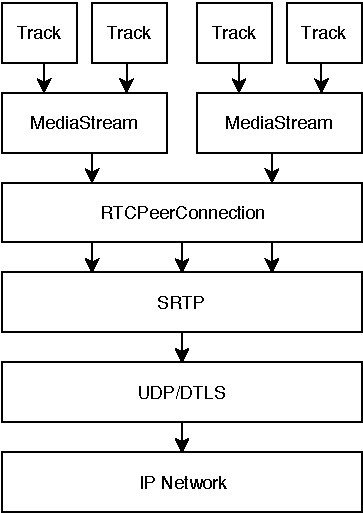
\includegraphics[width=.5\textwidth]{graphics/media-stream-pipeline.pdf}
\caption{Browser media streaming pipeline and network stack}
\label{fig:pipeline}
\end{figure}

\subsubsection{WebRTC Media}
\label{subsec:webrtc-media}

"WebRTC provides media acquisition and delivery as a fully managed service: from camera to the network, and from network to the screen", as \citet[\S18.5]{high-performance-browser-networking} describes it. The browser provides a powerful, high-level interface to developers which allows streaming media from one peer to another. A \lstinline|RTCPeerConnection|, as defined by \citet[\S4.4]{webrtc-w3c}, can add streams on the producer side as well as receive streams on the consumer side. Under the hood, however, browsers must perform a complex transmission process (see \cref{fig:pipeline}). Because \gls{webrtc} runs on top of the \gls{udp}, the connection is unreliable by default. However, for live streaming applications, timeliness at the cost of video quality is deemed more important than a persistent quality at the cost of delays and stutter \cite[\S18.3]{high-performance-browser-networking}. The \gls{webrtc} network engine uses a stack of two transport protocols to deliver the best possible media stream across a constantly changing connection. \Gls{srtcp} is used to measure and exchange metadata about package loss, sequence errors, jitter and more between the two peers. Those statistics influence how the browser chooses appropriate quality and codec settings. \gls{srtp} on, the other hand, is used to transmit the encoded audio and video byte stream.

\subsubsection{HTTP Streaming}
\label{subsec:http-streaming}

With the adoption of \gls{html} 5, online video streaming has moved from plugin-based approaches like Adobe Flash\footnote{\label{adobe-flash}Adobe Flash Player. URL: {https://www.adobe.com/products/flashplayer.html}} or Microsoft Silverlight\footnote{\label{silverlight}Microsoft Silverlight. URL: {https://www.microsoft.com/silverlight/Default}} to native, browser-based technologies. Namely, two competitors have emerged: \gls{hls} and \gls{mpegdash}. The former was developed by Apple, and although not being internationally standardized, \gls{hls} was adopted by some other vendors as well \cite{caniuse-hls}. The successor \gls{mpegdash} has been standardized by \citet{iso-mpeg-dash} and does not require specific video codecs and has built-in \gls{drm} capabilities. What both have in common, is that they split media streams into short segments and use a manifest file to stitch them back together on the client side. This, plus the fact that they run on top of HTTP, make them work well on modern \glspl{cdn}, as \cite{hls-vs-dash} points out.

\subsubsection{Media Formats}

When considering the fragmented landscape of browser media streaming technologies, the actual media encodings being used are even more vendor and version dependent, as the compatibility table for in-browser playback at \cite{media-format-browser-compat} shows. For playback, common ground between browser vendors can be found with VP8 compression in a WebM container or H.264 in MP4. However, when trying to encode media recorded on-device, the set of supported formats is even smaller and, according to \citet[\S5.1]{webrtc-hacks-safari}, the broadest interoperability for video can be achieved with \textit{H.264}. Although, many mobile devices do not support hardware encoding of H.264. On the audio side, more modern and efficient formats like Opus and Vorbis have emerged. However, the widest support is still enjoyed by traditional MP3 \cite{media-format-browser-compat}.

\newpage
\subsubsection{WebRTC}\label{sec:webrtc}

In 2011, the \glsfirst{w3c} standardised the first version of \gls{webrtc} \cite{webrtc-w3c}. It was the first browser–native technology to enable \gls{p2p} connections for \gls{js} applications\footnote{To some extend, Adobe Flash and Java Applets already allowed \gls{p2p} connections, but required browser plugins primarily compatible with Desktop systems and are on their way to deprecation.}. Since then, adoption has spread to all major vendors \cite{webrtc-browser-compat} and its browser \glspl{api} have matured.

\gls{webrtc} is the only browser interface to the \gls{udp} transport layer. In contrast to the \gls{tcp}, which powers \gls{http} and \gls{ws} based communications, \gls{udp} is a so called "null protocol" \cite[p. 36]{high-performance-browser-networking}. This means, \gls{udp} does not take any measures to assure 1) packets arrive in order, 2) packets arrive at all, 3) connections preserve state or 4) the network does not congest. Consequently, \gls{udp} requires a lot less overhead than \gls{tcp} and performs better at time–sensitive applications like live media streaming.

\paragraph{Connection Negotiation}\label{par:webrtc-con-negotiation}
Unlike web servers, web clients engaging in \gls{webrtc} connections are not publicly reachable by default. They are often connected to private networks and do not listen on ports on their network interface.
Hence a client needs to be informed of an inbound connection \textit{out-of-band}. With \gls{webrtc}, such connection intents are formalised by the \glsreset{sdp}\gls{sdp}. \gls{sdp} "is used to describe the 'session profile,' which represents a list of properties of the connection: types of media to be exchanged (audio, video, and application data), network transports, used codecs and their settings, bandwidth information, and other metadata" \cite[p. 323]{high-performance-browser-networking}.
The \gls{sdp} payload \cite[\S5]{sdp-rfc} can be exchanged through any application-specific channel. Many \gls{voip} systems use the \gls{sip}, while many public telephone networks use \gls{isup} \cite[p. 321]{high-performance-browser-networking}. Moreover channels like \gls{ws}, Bluetooth or even QR Codes could be used.

\begin{figure}
\centering
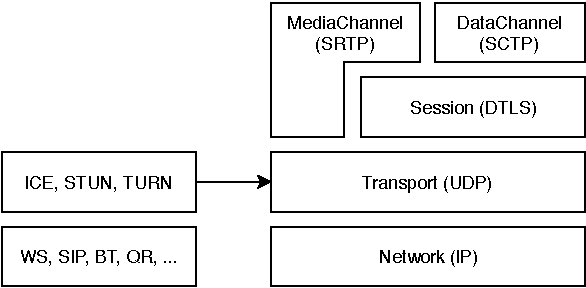
\includegraphics[width=0.75\textwidth]{graphics/webrtc-proto.pdf}
\caption{WebRTC stack, simplified from \citet[p. 316, fig. 18.3]{high-performance-browser-networking}}
\label{fig:webrtc-proto}
\end{figure}

\subsubsection{ICE Handshake}
What makes \gls{p2p} connection establishment so complex, is the broad employment of \gls{nat} devices. Most consumer and commercial networks as well as \glspl{mno} use \glspl{nat} to let clients inside a local network interface with the global internet.

Local devices establish connections to remote devices (like servers or peers) and the \gls{nat} maps their local \gls{ip} address and port tuple to a tuple consisting of the \gls{nat}'s \gls{ip} and a different port. If the \gls{nat} then receives a packet from the remote device on that port, it knows where to route it in the local network. This way, multiple devices can share a single \gls{ip} and are unreachable from the outside unless they initiated the connection. There are two basic categories of \glspl{nat} devices: symmetric and cone. The former will assign the external port randomly for any pair of local and remote device. This makes it impossible for a \gls{nat}ed device to determine its address using a stun server and pass it to a peer, because the peer will have a different \gls{ip} address and the \gls{nat} will reject the connection. The latter type, cone \glspl{nat} can have restrictions on ports or remote addresses, but will generally assign a static port to local devices.

So, to establish a connection between two peers through a cone \gls{nat}, each peer would have to find out its public \gls{ip} address and the port its \gls{nat} exposes for it. The \glsreset{stun}\gls{stun} standardise how a devices can contact a dedicated public server and receive said public \gls{ip} and port. Optionally, the \gls{stun} request can be encrypted and be sent over \gls{udp} or \gls{tcp}.

However, in case of peers behind a symmetric \gls{nat}, the connection negotiation with an address reported by a \gls{stun} server would fail. To combat this issue, \gls{webrtc} applications can use \gls{turn} servers to relay connections to remote peers. This is a non-optimal solution, since it requires costly bandwidth and potentially defeats the purpose of \gls{p2p} solutions. In cases of user–generated content, like video-conferencing, it may nevertheless be the only option.

In a third scenario, the peers would share an \gls{ip} address space. The preferable routing would then be neither of the above, but a direct connection without \gls{nat} traversal.

\vref{fig:webrtc-handshake} shows an example of one peer behind a \gls{nat} and one publicly reachable peer establishing a connection through the \gls{ice} handshake.

There are many possible network constrains that can influence the \gls{webrtc} connection setup, like firewalls and \gls{vpn} configurations. The problem is, that client-side applications cannot know which network scenario is applicable to their current connection attempt and have to find out by trial and error. The process of gathering routing "candidates" and testing them in order of ascending complexity is referred to as \glsreset{ice}\gls{ice} \cite{ice-rfc}. Most modern browsers implement \gls{ice}—at least partially—in their \gls{webrtc} \gls{api} \cite{webrtc-browser-compat}. While \gls{ice} makes the connection process more reliable it can lead to significant wait times for users. A draft by \citet{trickle-ice} proposes a standard called \textit{Trickle} for aggregating candidates asynchronously on connection initiator and target, thus accelerating the connection establishment considerably.

\paragraph{Protocol Stack}\label{par:webrtc-stack}
The \gls{webrtc} standard builds upon various proven protocols, that have already been in use by other telecommunication systems. Along dedicated media streaming, \gls{webrtc} also offers a data channel, that applications can use to exchange arbitrary messages. Media and data is sent over two different transmission protocols: \glsreset{srtp}\gls{srtp} and \glsreset{sctp}\gls{sctp} respectively. \vref{fig:webrtc-proto} visualises the stack of protocols in use. Both, \gls{srtp} and \gls{srtcp} packets, are transported via \gls{udp}. To overcome the lack of features (in comparison to \gls{tcp}), the \gls{webrtc} stack provides a set of tools: encryption can be achieved through \gls{dtls} and in-order delivery and transmission guarantees can be configured and are enforced in the application space, i.e. by the \gls{webrtc} browser implementation \cite[p. 319]{high-performance-browser-networking}.

\begin{figure}
\centering
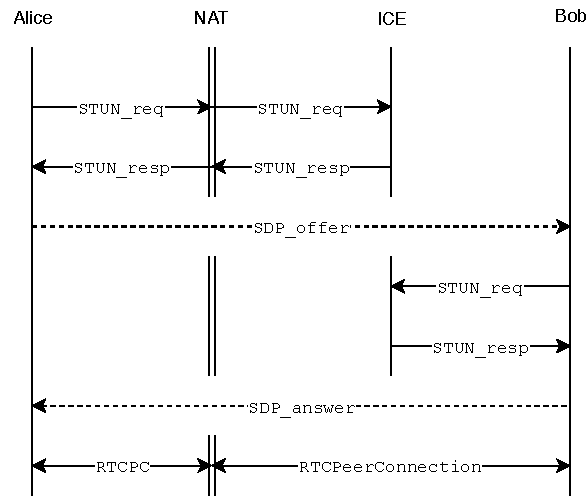
\includegraphics[width=0.75\textwidth]{graphics/webrtc-handshake.pdf}
\caption{WebRTC handshake example with Alice behind a \gls{nat} device and Bob with a public \gls{ip}. The dashed line represents \textit{out–of–band} communication.}
\label{fig:webrtc-handshake}
\end{figure}

\newpage

\newpage
\section{Network}
Devices that are exchanging data are connected with each other and form a network. The ability of a device to connect one to another is provided by the network interface of a device. 

The network interface can use the \gls{ip}. Before a client can send data it needs to know about the presence and how to address the other device. Each device has a unique address inside the network which is called IP-Address. The IP-Address can be assigned either by a \gls{isp}, a \gls{dhcp} Server or it can have a static one in a local environment. 
Data is transmitted in form of IP-Packets. The IP-Packet has the IP-Address of the sender and of the receiver and next to other fields the actual payload \cite{roberts}.

To transfer an IP-Packet from one device to another a router is needed which connects two networks and is forwarding packets either inside the local network or to the other connected network as described by \cite{shuler2002}.
Each device is registering itself at the router. The router then stores the IP-Address in a routing table. All devices known by the router are representing the local network. 

When the router receives an IP-Packet it looks up the receiver IP-Address in its routing table and is then forwarding the packet to the receiver when an entry exists.
When no entry exists the packet is forwarded to another network. The router of the other network is taking care of it. The other router is repeating the process until some router knows the receiver.
To prevent infinite hopping of IP-Packets each packet has a \gls{ttl}. The \gls{ttl} is decreased on each hop until it reaches zero where it is not forwarded to the next router anymore. 

To enable a reliable and secure way how packets are transmitted from one device to another more mechanisms are needed e.g. handling packet loss. 
To provide a common basis how to achieve that, the \gls{osi} model has been specified.
The \gls{ip} is only one layer out of six other layers.

\section{OSI-Model}
\blockquote{The purpose of this Reference Model of Open Systems Interconnection is to provide a common basis [...] of systems interconnection, while allowing existing standards to be placed into perspective with the overall Reference Model} as specified by \citet{ISO1064-osi-model}. Seven abstract layers are specified and each of them shall provide functionality without depending on other layers. This means that a layer has to be implemented in a transparent manner meaning that implementation details shall be hidden for other layers and expose an interface so it can be used by a layer above.

The seven layers of the OSI-Model are shown in \cref{fig:osimodel}. Data that is received by a device runs through all layers starting at layer one and leaving at layer seven where it will be consumed by an application. Just as the data is processed on receive, the same steps have to be taken before it can be transmitted, but in reverse order. This means data enters at layer seven and leaves the device in form of bits at layer one.

\begin{figure}
\centering
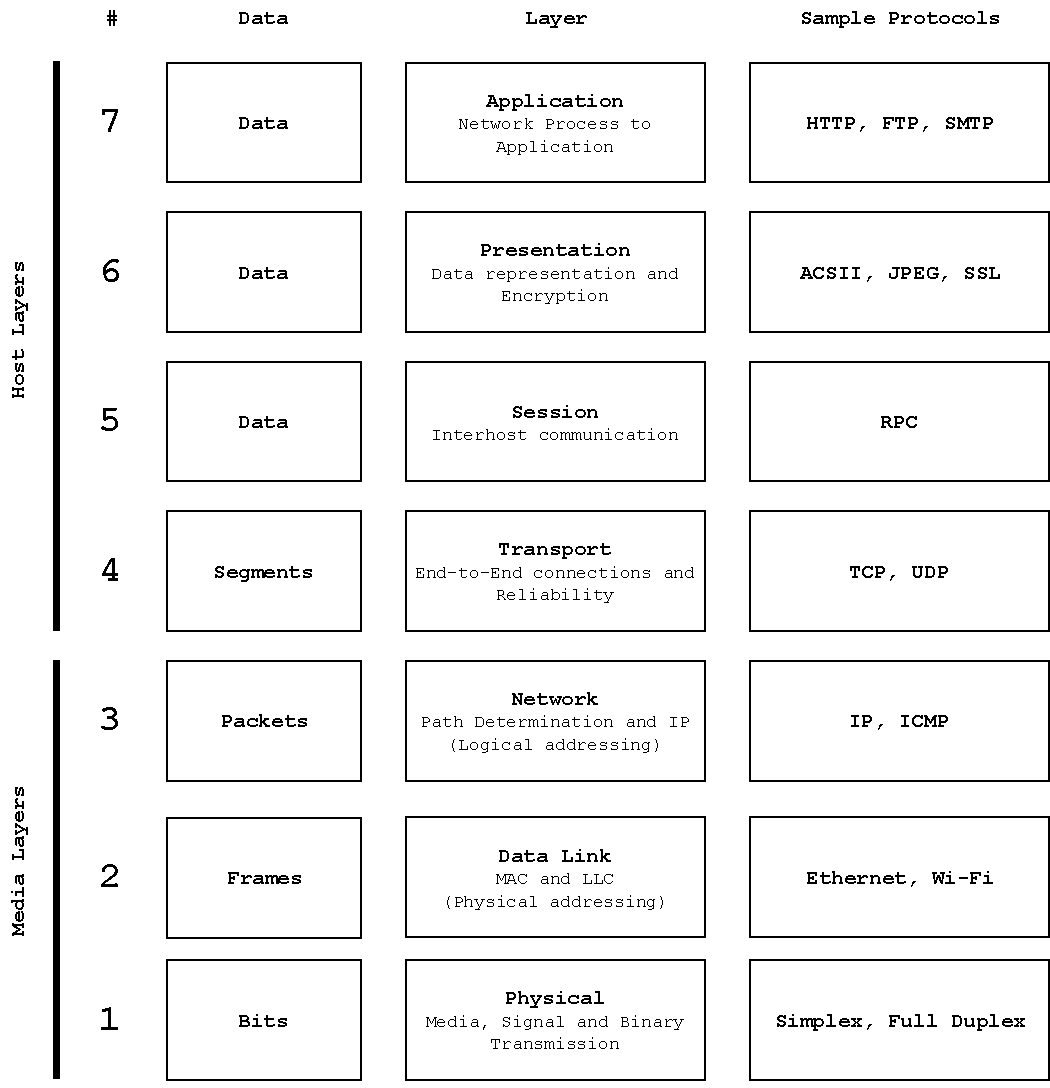
\includegraphics[width=.5\textwidth]{graphics/osi-modell.pdf}
\caption{OSI-Model (adapted from \citet{wiki:osi-model})}
\label{fig:osimodel}
\end{figure}

\subsection{Application Layer}
Incoming data\newline
Device applications like browsers, email clients, calenders,... are interacting only with this layer. The application layer provides an interface that comes from the underlying protocol like \gls{http} for Browser applications or \gls{smtp} for E-Mail applications. The data is in a consumable state and it is up to the application what to do with it.

Outgoing data\newline
Similar as for incoming data the application layer is also the entry point for device applications to send data using the protocol of the application layer like \gls{http}. 


\subsection{Presentation Layer}
Incoming data\newline
Preparing the data and making it consumable for the application layer is the task of the data layer. 
Hence, data has to be decrypted when it is encrypted, decompressed and put into the right format by decoding it.

Outing data\newline
Outing data can be encrypted, compressed and encoded by this layer.

\subsection{Session Layer}
Keeping the session and connection between two devices is one of the responsibilities of the session layer. It can also keep track of transmitted data so in case the connection is interrupted it can continue where it left off e.g. when a file transfer is interrupted the file does not be re-transmitted from the first byte. 

\subsection{Transport Layer}
Incoming segments\newline
The transport layer is responsible for reassembling incoming segments and putting them into the right order, for error handling e.g. deal with lost packets and to determine the optimal connection speed how to communicate with the other. 
The two main protocols are \gls{tcp} and \gls{udp}

Outgoing data\newline
Data that is sent is segmented into smaller chunks and further processed by the underlying protocol, e.g. \gls{tcp} adds a sequence number to each segment.

\subsection{Network Layer}
Incoming packets\newline
Incoming Packets are routed towards the receiver when the device is not the receiver and the receiver is not in the same network. Otherwise packets are  reassembled into segments and handed over to the transport layer.

Outgoing segments\newline
For outgoing segments the network layer is responsible for creating packets and routing them towards its destination.
The well known \gls{ip} is operating on this level. Segments provided by transport layer  are segmented into packets. Each packet gets a \gls{ip} packet header that contains the address of the sender, the adress of the receiver, a \gls{ttl}, the protocol with its version and other fields \cite{rfc791-ip}. The packets are then routed via routers towards the destination when the receiver address exists somewhere.

\subsection{Data Link Layer}
Incoming frames\newline
Tasks of this layer involve segmenting packets into frames and transmitting them within the same network.
Common networking components that are operating on this level are switches, hubs and network interface cards \cite{simoneau2006}.

Outgoing packets\newline
Packets received from the network layer are segmented into frames 

\subsection{Physical Layer}
The physical layer is the layer where the actual transport happens on a physical connection in form of electrical or optical signals.
Outgoing frames are transformed into bits (0,1) which can be represented as a signal.
Incoming bits are reassembled into frames and handed over to the data link layer.


\section{Overlay Network}
\begin{figure}[htb!]
\centering
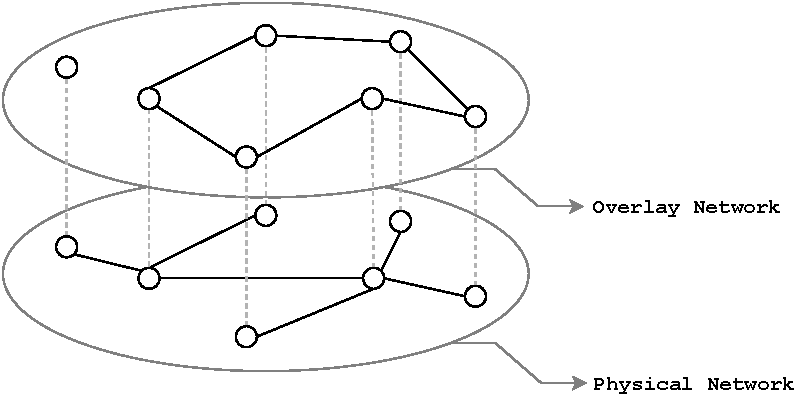
\includegraphics[width=.5\textwidth]{graphics/physical-vs-overlay-network.pdf}
\caption{Physical and overlay network example}
\label{fig:overlay}
\end{figure}
Devices that are connected with each other form a physical network. On top of that network a virtual network can be constructed—a so called overlay network. The overlay network only cares about who is part of the network and not how the partner is reachable. 
While the physical communication has physical links between devices, the overlay network makes usage of virtual edges to connect devices that are not physically connected with each other. When a device wants to connect to a device that is not physically connected the overlay network can use indirect connections. That means when \textit{A} is connected to \textit{B} and \textit{B} is connected to \textit{C}, the overlay network allows \textit{A} to send data to \textit{C} via \textit{B}.
\cref{fig:overlay} shows a sample physical network and its derived sample overlay network.

As the underlying physical is transparent to the developer, the overlay network offers a huge design flexibility. The developer is free to chose her own network topology and protocol to use e.g. \gls{tcp} or \gls{udp}. However, the developer is responsible to maintain the virtual edges. This means when a device leaves the network, the overlay network has to be updated accordingly e.g. establish a replacement edge.

\section{Overlay Network Topologies}
The most common overlay network topologies are shown in \cref{fig:overlay-topologies}. In a centralised topology all devices are connected to one central device. A typical centralised example is the internet. The central device is a server and all other devices exchange information with that device. Advantages of this topology that it is easily manageable and the maintainer has full control over it. Thus, the provided information is always up to date and the maintainer can control who has access to it. However, a centralised network can not grow endlessly but only as big as the central device can handle the traffic. There is also a single point of failure. When the central device is not available anymore the whole network is offline.
\begin{figure}[htb!]
  \centering
    \subfloat[Centralised]{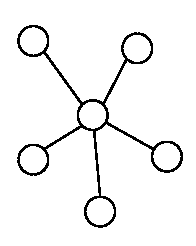
\includegraphics[width=0.25\textwidth]{graphics/overlay-network-centralised.pdf} \label{fig:overlay-topologies-a}}
    \subfloat[Hierarchical]{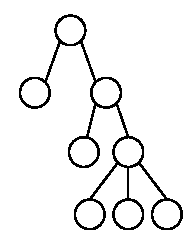
\includegraphics[width=0.25\textwidth]{graphics/overlay-network-hierarchical.pdf} \label{fig:overlay-topologies-b}}
	\subfloat[Decentralised]{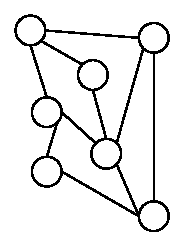
\includegraphics[width=0.25\textwidth]{graphics/overlay-network-decentralised.pdf} \label{fig:overlay-topologies-c}}
	\subfloat[Hybrid]{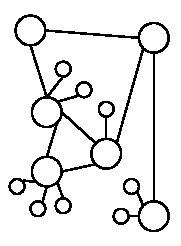
\includegraphics[width=0.25\textwidth]{graphics/overlay-network-hybrid.pdf} \label{fig:overlay-topologies-d}}
	\caption{Common overlay network topologies}
\label{fig:overlay-topologies}
\end{figure}

A typical usecase for an overlay network is a \gls{p2p} environment.

\section{Peer-to-Peer Network}

\newpage
\section{Mesh Network}
\label{chap:mesh-network}
In a centralised environment each client communicates only with the central client. Therefore clients do not have to know other clients.
Clients in a decentralised network do not have a central counterpart. Thus a client has to discover other client and establish connections to them.

A more than 15 year old standard to achieve this is \gls{ip} multicast. The multicast concept operates on OSI-Layer 3 and is based on groups. Anyone can create a group with a unique address where others can receive packets from and send packets to \cite[pp. 484-485]{tanenbaum_wetherall_2011}. Based on ping messages the liveliness of group members is periodically checked. When a packet is addressed to a group the router has to duplicate packets and broadcast to all clients. 
The use cases for multicast are unlimited like group chats, conference calls or tv broadcasting.
However, due to technical limitations, like scaling issues and limited address space, it did not prove to be successful \cite{multicast}.

As multicast is not widely deployed, a decentralised network has to be constructed as a overlay network on OSI-Layer 7—the application layer \cite[\S1]{multicast-problems}.

An overlay network where clients are connected with each other in an autonomous manner is called Mesh Network. The easiest approach is to connect all the clients with each other, which would result in a fully connected mesh network. However, with a growing number of participants this approach becomes unfeasible because each client can only handle a limited amount of connections.

Due to this limitation a client can only connect to a subset of the total available clients. To reach clients without a direct connection it has to make use of other clients as forwarders. Therefore packets have to be routed through the network by a routing protocol.

\subsubsection{Broadcasting Routing Protocols}
In the easiest scenario of a decentralised network a client is broadcasting a packet to all other clients in the network. For this scenario the client does not need to know about the presence of other nodes besides the clients it is directly connected with.

\paragraph{Flooding}\label{flooding}
The client sends a packet to all directly connected clients. Those clients are forwarding the received packet to all their directed clients that are not the last sender of the packet. Eventually, all the clients in the network will receive the packet. 

The process of forwarding a packet to all direct connected clients is one of simplest message routing algorithms and called \textit{Flooding} \cite[p. 368]{tanenbaum_wetherall_2011}

To prevent infinite hopping broadcast packet it has to be dropped at some point, meaning that it is not forwarded anymore.
One option to achieve this is, is to set a \gls{ttl} on the packet. Each hop that is receiving a packet is decreasing the \gls{ttl} by one. As long as the \gls{ttl} is greater than zero the packet is broadcasted otherwise it is dropped. One issue that arises by a \gls{ttl} is that it may not reach all the clients in the network because it is discarded before.

When it is necessary that all clients get the packet another option is to set an incremental increased sequence number on the packet.
A client that receives a packet with a sequence number can check whether it has received a packet with that sequence already. When the sequence number is new it stores the sequence number for that message and re-broadcasts the packet. Otherwise the packet is dropped by the client.

\begin{figure}
\centering
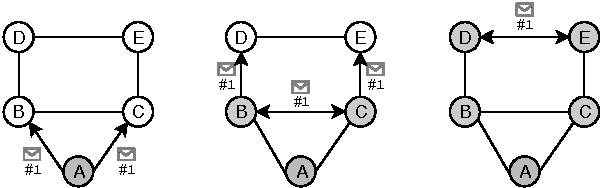
\includegraphics[width=1\textwidth]{graphics/flooding-with-sequence.pdf}
\caption{Flooding a packet with a sequence number}
\label{fig:flooding}
\end{figure}

\cref{fig:flooding} shows the flow of a packet that has been dispatched by \textit{A} with the sequence number \textit{\#1}. \textit{A} is increasing its own sequence number for the next packet. \textit{B} and \textit{C} receive the packet and as the sequence number is unknown to them they re-broadcast the message to their connected clients (\textit{B}$\rightarrow$\textit{C}\&\textit{D},  \textit{C}$\rightarrow$\textit{B}\&\textit{D}). \textit{B} and \textit{C} receive a packet with a sequence number both have already seen, so the message is discarded. The sequence number prevents an infinite back and forth hopping that would otherwise clog the network.

The Flooding mechanism is tremendously effective when the task is to reach all clients in the network because it will find the shortest path to all clients due to the fact that all paths are tried.
However it also generates a lot of overhead traffic. As seen in \vref{fig:flooding}, \textit{B} $\leftrightarrow$ ︎\textit{C} and \textit{D} $\leftrightarrow$ \textit{E} are sending the packets back to each other as they do not know that the counterpart has seen the packet already. The packet is dropped but still it is a unnecessary transmission.

\paragraph{Gossiping}\label{gossiping}
\largepage
Gossip Protocols take human nature and epidemics as a role model how to spread information inside the network. 
In a nutshell it works similar to \textit{Flooding} but instead of sharing a packet with all direct connected clients only a subset is selected where the packet is transmitted to. There are different selection strategies like random selection or selection based on a heuristic. 
Clients that were \say{infected} repeat the same procedure. This is almost as effective as \textit{Flooding} as \citet{riviere_voulgaris_2011} phrase it \say{Making a random selection out of a random subset of all nodes is equivalent to making a random selection out of \textit{all} nodes.}
However, as the there is a client selection it is not as efficient as \textit{Flooding} in terms of time until the packet has reached all clients.

\citet{Jelasity2011} describes two models of \textit{Gossip} SI and SIR:

\begin{itemize}
\item susceptible (S): The node does not know about the update
\item infected (I): The node knows the update and is actively spreading it
\item removed (R): The node has seen the update, but is not participating in the spreading process (in epidemiology, this corresponds to death or immunity)
\end{itemize}
\cite[\S1.2.2]{Jelasity2011}

Those are the three states a client can have when a \textit{Gossip} packet is spread through the network.

SI:
In the SI-Model a node is in \textit{\textbf{S}usceptible} state until it receives a \textit{Gossip} packet from another client. On receive it switches into the \textit{\textbf{I}nfected} state and starts spreading it in a fixed interval to selected peers. This is the \textit{push}-variant of the SI-Model. There is also a \textit{pull}-variant where the client act passively and only asks neighbour clients whether they have a \textit{Gossip} packet. A third variant is the \textit{push-pull}-variant where the client is actively spreading the packet as soon as it is in the \textit{\textbf{I}nfected} state but also asks neighbours whether they have a \textit{Gossip} packet.  
\begin{Listing}
\begin{lstlisting}[multicols=2,basicstyle=\tiny,basicstyle=\footnotesize\ttfamily,xleftmargin=3em]
loop
  wait()
  p <- random peer
  if push and in state I then
    send update to p
  end if
  if pull then
    send update-request to p
  end if
end loop

procedure ONFEEDBACK(m)
  switch to state R with prob. 1/k |\label{line:SIROnFeedback}|
end procedure
procedure ONUPDATE(m)
  if in state I or R then
    send feedback to m.sender |\label{line:SIRfeedback}|
  else
    store m.update // now in state I
  end if
end procedure

procedure ONUPDATEREQUEST(m)
  if in state I then
    send update to m.sender
  end if
end procedure
\end{lstlisting}
\caption{SIR from \cite[\S1.2.2.2]{Jelasity2011}}
\label{lst:SIRAlgo}
\end{Listing}

SIR:
SIR works like SI only that it has a third state \textit{\textbf{R}emoved}. While the SI-Model will never terminate spreading the \textit{Gossip} packet, thus producing a lot of unnecessary traffic, SIR terminates the spreading as soon as the node enters the \textit{Removed} state.

\Cref{lst:SIRAlgo} shows the basic functionality of SIR. 
When the client receives a \textit{Gossip} packet it has already seen, it sends feedback to the sender of the packet (line \ref{line:SIRfeedback})
On feedback a client that has send a \textit{Gossip} packet can switch to state \textit{Removed} (line \ref{line:SIROnFeedback}). In the described algorithm this happens with a probability of 1/\textit{k}, \say{where the natural interpretation of parameter k is the average number of times a node sends the update to a peer that turns out to already have the update}\cite[\S1.2.2.2]{Jelasity2011}. When the client is in state \textit{Removed} it will not send any updates to other clients anymore

\subsection{Client Discovery}
The previous described routing protocols rely on the assumption that a node does not need to know the whole network. They only need to know their directly connected clients in order to forward packets.
For many scenarios where a Mesh Network is deployed the only knowledge of direct clients is not enough. In fact, in many scenarios a bigger picture of the network is needed or at least the knowledge about the presence of a client. This involves client discovery. However, a client that has discovered other clients does not need a connection to them, it only needs to know that the client is somehow reachable.
Client discovery, path discovery and maintenance are tasks that \textit{Reactive Routing} and \textit{Proactive Routing} protocols are dealing with.

\subsection{Reactive Routing}
Reactive protocols act passively, meaning that they are not actively looking for clients but only when a packet has to be forwarded to an unknown client.
When a packet is received by a client that is not meant to be the receiver, the client has to forward the packet. In case it does not know any routing information how the receiver can be reached it has to acquire routing information. 
To acquire routing information it can make use of \textit{Flooding} (\cref{flooding}) and flood a route request to its directly connected clients. \say{These neighbours forward the route request packet to their neighbours and this process goes on until either the target node or an intermediate node with a valid route to target node is located. Each node receiving a particular route request packet broadcasts it only once to its neighbours, and it discards the subsequent receptions of the same route request packet, to minimise routing overhead} as described by \citet[\S1.3]{Mukhija_Arun}. 
Protocols that are reactive are for example AODV, DSR, TORA whitch are compared by \citet{kalwar_2010}

\subsection{Proactive Routing}
In comparison to the passive acting reactive protocols the proactive ones are actively gathering information about the network by periodically sending \textit{Ping}-Packets. Each client is maintaining a routing table. When it receives a (\textit{Ping})-packet from an unknown client the client is added to the routing table with the last hop neighbour as originator. The client now can reach the added client via the originator. 
There are different approaches how the \textit{Ping} are propagated through the network. Most of them also rely on \textit{flooding} or \textit{gossiping}.
A expiration mechanism has to take care of removing clients where no \textit{Ping}-Packet has been received for a defined number, otherwise a client will stay in the table for ever, even though it has lost its connection to the network a long time ago.

\subsection{OSLR}\label{sec:mesh-oslr}
\gls{olsr} is a proactive routing control which is optimising the amount of \textit{HELLO} packets needed to discover other clients in the network.
A client that is directly connected to another client is seen as \textit{1-Hop Neighbour}. \textit{1-Hop Neighbours} are exchanging continuously \textit{HELLO} packets where they also include all their \textit{1-Hop Neighbours}.

On receive the client is adding all neighbours that are included in the \textit{HELLO} packet as \textit{2-Hop-Neighbours} in their neighbour table. Excluding all direct peers from \textit{2-Hop-Neighbours} are the \textit{Strict-2-Hop-Neighbours}.
Based on the list of clients the client knows it is now selecting \glspl{mpr}. \Glspl{mpr} are \say{selected such that it covers (in terms of radio range) all symmetric strict 2-hop nodes.}\cite[\S1.4]{rfc-oslr}. A client that has selected a \gls{mpr} is a \textit{MPR-Selector}. Clients are \say{upgraded} to \gls{mpr} by the \textit{HELLO} packets that can also include a list of selected \glspl{mpr}.

\Glspl{mpr} are disseminating \gls{tc} packets to all their clients with the list of their \textit{MPR-Selectors} and their sequence number that represents the sequence at which the client was selected as \gls{mpr}.
Clients receiving the \gls{tc} packet are setting up a topology table with the last-hop neighbour, the selected \gls{mpr} and the sequence number of the selected \gls{mpr}.

Each client is maintaining also a \textit{Routing table} which aggregates the \textit{Neighbour table} and the \textit{Topology table} into one. Entries of the \textit{Routing table} are all the clients a client can address as long as they are not leaving the network. 

Based on the \textit{Routing table} a client tries to find the optimal path to each entry. \citet[\S4.4]{jacquet_muhlethaler_clausen_laouiti_qayyum_viennot} describe in detail how the routing table is calculated.

\subsection{B.A.T.M.A.N}\label{sec:batman}
Another approach is the \textit{B.A.T.M.A.N} Protocol which stands for \textbf{B}etter \textbf{A}pproach \textbf{T}o \textbf{M}obile \textbf{A}d hoc \textbf{N}etworking and is developed by the Freifunk Community.

It is making use of \textit{gossiping}(\ref{gossiping}) to disseminate \glspl{ogm} through the network. Each client is sending a \gls{ogm} to their direct neighbour. \say{These neighbors are re-broadcasting the OGMs according to specific rules to inform their neighbors about the existence of the original initiator of this message and so on and so forth. Thus the network is flooded with originator messages.} as described in the concept of \citet{batman}.

\Glspl{ogm} contain, among other fields \cite[\S2]{tobias_hardes}, the address of the sender, the address of the last sender, a sequence number, a \gls{ttl} and a \gls{tq}. 
Once a client receives an \gls{ogm} it adds the sender to its own routing table and forwards the packet to all its directly connected clients when some criteria a met. 
The routing table entry has, among others\cite[\S2.1]{tobias_hardes}, the fields originator address, next-hop address, potential next hop addresses, last-seen and \gls{tq}.

Unlike other protocols, where the packet is not sent back to the sender, B.A.T.M.A.N is also answering to the sender by sending the packet back. Those packets are \textit{Echo} pakets. By doing so it each client is calculating the \gls{tq} to each directly connected client by counting the total amount of \gls{ogm} packets received from that client—\gls{rq} and the amount of \textit{Echo}-\gls{ogm} packets received—\gls{eq}. 
The packets are counted by using a sliding window \cite[\S3.4]{tanenbaum_wetherall_2011} with a fixed size. \cref{fig:sliding-window} shows a sample sliding window with size 2. 

Each client initialises a sliding window for outgoing \glspl{ogm} and for incoming \glspl{ogm} to each of its directly connected clients. When it dispatches an \gls{ogm} the outgoing sliding window sequence is increased by one. By moving the sliding window all values that are out-of-window are removed.

\begin{figure}
\centering
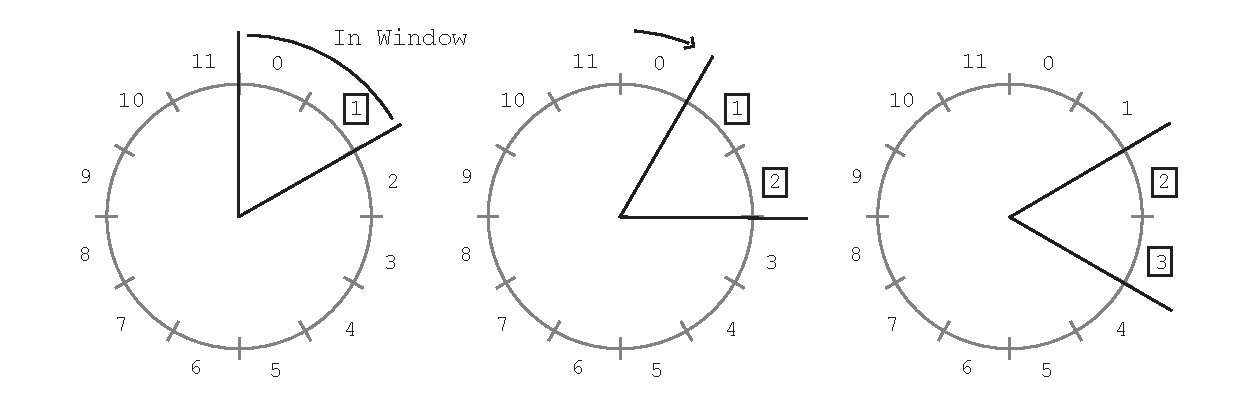
\includegraphics[width=1\textwidth]{graphics/sliding-window.pdf}
\caption{A sample sliding window}
\label{fig:sliding-window}
\end{figure}

When an \gls{ogm} is received the client checks whether it is one that it has send, thus a \textit{Echo} packet. When it is an \textit{Echo} packet it checks the outgoing sliding window whether the sequence number is in-window. If it is, the sequence number is added to the sliding window. By counting all values in the sliding window the client obtains the \gls{eq}. 
In the other case the client checks the incoming sliding window. When the sequence number is out of window it adds the sequence, slides the window to the new sequence number and drops all sequences out of window. This results in the \gls{rq}.

\say{With both values, it is possible to determine, whether the link is a bidirectional one and to create a metric to compare different links.}\citet[\S2.3.3]{tobias_hardes}. The value is determined by dividing the \gls{eq} through \gls{tq}.

\begin{equation}
\label{eq:transmit_quality}
\gls{tq} = \frac{\gls{eq}}{\gls{rq}}
\end{equation}

When the \gls{tq} is 1 it means that the outgoing connection to the other client is as good as the incoming. A value less than 1 means that packets got lost on the way.

A client dispatching an \gls{ogm} is setting a sequence number based on the outgoing sliding-window an initial \gls{tq} for the \gls{ogm} and an initial \gls{ttl} (initial \gls{tq} and \gls{ttl} are both fixed values). 

On receive of an \gls{ogm} the client is checking whether the sequence number is out of the receive sliding-window. In case it is not it means the client has already received the packet from another client so it does not have to be further broadcasted.

For a first-time seen sequence number the client is processing the \gls{tq} value of the \gls{ogm}. It is multiplying the calculated \gls{tq} to the last sender of the packet (witch results in a value between 0 and 1) with the current value of the packet. Then a hop penalty is subtracted (which is a configurable value) to punish routes with many hops because each hop in between could loose connectivity at any time.

\begin{equation}
\label{eq:ogm_quality}
new\_ogm\_tq = ogm\_tq * last\_hop\_tq * hop\_penalty
\end{equation}

When the resulting \gls{tq} is greater than zero it adds or updates the sender of the \gls{ogm} in its routing table with the \gls{tq} value of the \gls{ogm} when the originator is not a direct neighbour. When also the \gls{ttl} is greater than zero it broadcasts the \gls{ogm} to its neighbours.
The \gls{tq} and the \gls{ttl} prevent that the packet are limiting the traffic impact of one \gls{ogm} otherwise the whole network would eventually get \glspl{ogm} of any other peer and the traffic impact would be to high.

The \gls{tq} of the Routing-Table helps a client to determine which is the best router for a message.

\begin{figure}
\centering
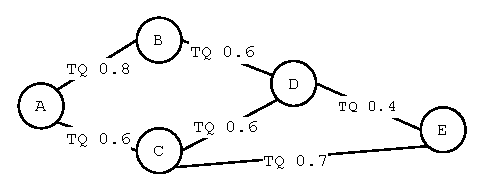
\includegraphics[width=0.7\textwidth]{graphics/batman.pdf}
\caption{Sample graph}
\label{fig:sample-graph-with-tq}
\end{figure}

\vref{fig:sample-graph-with-tq} shows a sample graph with nodes that have calculated the \gls{tq} to their direct neighbours. Needless to say but every node only knows the \gls{tq} so for example \textit{Node A} does not knows that the \gls{tq} between \textit{Node E} and \textit{Node F} is 0.4. The \gls{tq} for the multi–hop neighbours has to be calculated by exchanging \gls{ogm}.

\vref{tbl:sample-tq-table} shows the deviated routing table of \textit{Node A}

\begin{table}[htb!]
  \centering
  \begin{tabu} to \textwidth {X[c]X[c]X[c]}
		\toprule
    		\textbf{Originator} & \textbf{Next–Hop} & \textbf{TQ} \\
		\midrule
		B & B & 80.0 \\
		B & C & 17.5\\
		C & C & 60.0 \\
		C & B & 23.3 \\
		D & B & 43.2\\
		D & C & 32.4\\
		E & B & 15.5 \\
		E & C & 37.8 \\
		\bottomrule 
	\end{tabu}
\caption{Sample routing table for \textit{Node A} based on \cref{fig:sample-graph-with-tq}}
\label{tbl:sample-tq-table}
\end{table}

\paragraph{Example TQ for Node E}
For the calculation of the the \gls{tq} value an initial \gls{ogm}-\gls{tq} of 100 and a \textit{hop penalty} of 0.9 is given.
The \gls{tq} of \textit{Node E} arises out of the path taken by the \gls{ogm}.
When \textit{Node E} dispatches its \gls{ogm} it is taking the path E$\rightarrow$C$\rightarrow$A and E$\rightarrow$D$\rightarrow$B$\rightarrow$A. \vref{eq:tq_example} shows how the \gls{tq} is calculated.

\begin{equation}
\label{eq:tq_example}
\begin{aligned}
\gls{tq} _{next-hop-C} = & \overrightarrow{EC} (100 * 0.7 * 0.9) * \overrightarrow{CA} (0.6) = \textbf{37.8} \\
\gls{tq} _{next-hop-B} = & \overrightarrow{ED} (100 * 0.4 * 0.9) * \overrightarrow{DB} (0.6 * 0.9) * \overrightarrow{BA} (0.8) = \textbf{15.5}
\end{aligned}
\end{equation}

By sorting the table by \gls{tq} \textit{Node A} would send its message via \textit{Node B} because the \gls{tq} is better than the one of \textit{Node C}.

\newpage
\section{Peer–to–Peer}
\section{Peer-to-Peer}
In a Peer-to-Peer system a peer acts as booth client and server at the same time, meaning that it consumes content but also provides content for others. Unlike the traditional server-client model where the server acts as the single point of content distribution, Peer-to-Peer systems are not build on a centralised architecture so each peer can act autonomously and provide content to anyone else in the system.

As there is no central point there is also no single-point of failure and no single point as bottleneck. Thus a Peer-to-Peer can scale much better as described by \citet[\S1]{newscast-gossiping}:
\say{A well-designed peer-to-peer network can easily scale to millions of processes, each of which can join or leave whenever it pleases without seriously disrupting the system’s overall quality of service}. \citet[\S7.5.4]{tanenbaum_wetherall_2011} even go a step further and say that peer-to-peer networks are \say{self-scaling}.
Due to its nature of design it is also hard to censorship or shut down a peer-to-peer network because there is no central entity that someone can take control of. Also there is no central database that someone could attack or that can be used to monitor people in order to sell the data to 3rd parties.

According to \citet{tanenbaum_wetherall_2011} Peer-to-Peer systems have become popular in 1999 with the introduction of Napster, a Peer-to-Peer music streaming service. However, as it was mainly used to share copy-right infringed material, it was shutdown by government soon after. Shutting down the service was possible because Napster was not a fully decentralised Peer-to-Peer system. A central server was used as an index server to store the relation of content and who is hosting the content. Peers interested in content were querying the index server and got addresses as a result of peers hosting the content matching to the search query. The content itself was exchanged in a peer-to-peer manner so the client opened a direct connection to the address and downloaded the content. By shutting down the index server the peers could not locate any content anymore. 

The hybrid approach of Napster, using an index server was their solution of the complex problem of content discovery in a decentralised Peer-to-Peer network.

\subsection{Content Discovery}
Finding or publishing content in a Peer-to-Peer network is not a trivial task. In fact, depending on the structure of the network, the size and the chosen search strategy it might be impossible to find content, even though it might exist somewhere.

To discover content there are two typical scenarios:
\begin{itemize}
  \item Searching for content with a search query
  \item Finding content based on an address
\end{itemize}

\paragraph{Searching}
As the name indicates searching is using a search query to query the network for content. When content exists the query returns a hit with the peers hosting the content. Peers are usually returned as addresses so a peer can connect to them.

In the example of Napster a user was publishing content by creating an entry on the index server with the meta descriptions of the content and its own address. Other peers were querying the index server with a search query. The index server looked up its own database for content matching the query. When content was available it returned the address of the peer hosting the content. 

An approach that gets rid of the central server is \textit{Flooding}. In this approach a query is flooded through all peers in the network until it finds a match. \textit{Gnutella} which has become popular soon after the shutdown of Napster was using this strategy.

The first version of the Gnutella Protocol was using \textit{Flooding} to disseminate a \textit{QUERY}-Packet through the network with the search query and a \gls{ttl}. When a peer does not have content matching the query it forwards the query to all its neighbours as long as the \gls{ttl} allows re-broadcasting. A peer that has content returns a query hit which is send back the same path as it came in \cite[\S4]{gnutella04}.

However as Gnutella became more and more popular scaling the system to support the growing amount of peers was crucial to keep the system alive. \say{LimeWire (a company promoting an enhanced Gnutella servent) suggested therefore the introduction of a two-level hierarchy: Ultrapeers (UPs) and Leaf
Nodes (LNs)} \cite[\S3.1]{gnutellaAnalysis}

By having a two-tier hierarchy the general \say{standby traffic} (traffic to maintain the overlay network) has been reduced.

Instead of flooding a \textit{QUERY}-Packet, a \textit{Leaf Node} is now only sending it to its \textit{Ultrapeer}. The Ultrapeers are connected with other Ultrapeers and have a distributed knowledge about content that is provided by Leaf Nodes. When an Ultra Peer finds a Leaf Node that is providing content for the search query it is returning the address back to the originator of the query. The Gnutella protocol is further explained and evaluated by \citet{gnutellaAnalysis} but for the scope of this thesis not relevant.

\paragraph{Addressing}
In another scenario (cf. \vref{chap:IPFS}) the client already knows the content identifier and has to find the host which is providing the content.

In the server-client system this is done by addressing the server via its IP address and a path (\gls{url}) e.g. \textit{1.2.4.5/file/thesis.pdf}. The server is then looking up its file system and is returning the content, in case it is available.

The Peer-to-Peer system does not have a central file system and it would be infeasible to have one, because that would mean that data from each peer would need to be replicated over all other peers.

So instead of using a \gls{url} a peer is addressing only the file because it does not matter where the file is stored. This approach also makes it possible that the same content can be stored on multiple peers.

To make the file addressable one option would be to use its file name. However the file name is just a meta information which can be changed. To generate a more unique identifier for a file, a better approach is to create a hash over the file content with a hash algorithm (e.g. SHA-256). As long as the file content does not change the hash will be always the same. The hash can be used as an address because it is unique for that specific file.

As the file is addressable by its content hash and as the same file can live on multiple peers other peers need to be able to find it in the network.

This is where the \glsfirst{dht} comes into play.

\subsubsection{\glsfirst{dht}}
As the name of the \gls{dht} indicates, it works like a hash table with a key–value pair but is distributed among multiple peers. An arbitrary value, that could be anything from an address to a file, is mapped to a key by using the hash function. The key space of the hash table is divided into buckets and distributed among the participants, each taking care of one bucket. This way, each participant is responsible for a bucket and does not need a global knowledge about all existing key–value pairs.

To assign a bucket to a peer, first of all the peer has to be uniquely identifiable as well. Thus each peer get an identifier from the same id-space as the keys from the hash table. This could be for example a hash over the \gls{ip} address of a peer with the same hash function that was used for the key-value hash e.g. SHA-256.

As the peer ids and the keys of the hash table are in the same id space, the table can be partitioned into buckets by a distance function. The value key has be the closest to a peer id and the value key has to be greater than the node key. Fulfilling both conditions means that a peer takes care of the key space from its own node id until its successor node id.

When a new node enters the network some of the key space has to be reorganised, but not the whole key space. In fact, only the key space between the peer that is considered as a previous peer and the new peer has to be reorganised. This makes the \gls{dht} quite efficient as the remaining key space stays unaffected. 

A peer leaving the network is removing all the content that it has been hosting. This is always a problem of Peer-to-Peer systems and the only way to prevent this is to replicate content over multiple peers. \citet[\S3]{chord} proposes some solutions how one could deal with it, such as \say{Coorparative Mirroring} or \say{Time-Shared Storage}.

Another condition to make the \gls{dht} work is that the participating peers have to form an overlay network so they can communicate with each other. This can be achieved for example with one of the routing protocols described in Mesh-Networking (\vref{chap:mesh-network}).

When a peer wants to enter content into the \gls{dht}, it generates the key for the content with the given hash function. The key is send together with the content to a known peer of the the \gls{dht} as a \say{store-request}. When the peer is responsible for the key space of the given key it stores the key with the content. Otherwise it redirects the \say{store-request} to one of its known peers, where the peer id is closer to the key of the \say{store-request}. This step is repeated until the \say{store-request} reaches the peer responsible for the key space.

Looking up content in the \gls{dht} works similar. A peer sends a \say{content-request} with a hash to a known entry point. When a peer is responsible for the key space or has stored the content by itself, due to a previous request, it returns the content. Otherwise it redirects the request to another peer where the peer id is closer to the hash of the \say{content-request}.

\subsubsection{\gls{dht} Implementations}
There are a several different \gls{dht} implementations out there like Chord \cite{chord}, Pastry \cite{pastry}, Tapestry \cite{tapestry} and Kademlia \cite{kademlia} to name just a few.
According to \citet[\S7.5]{tanenbaum_wetherall_2011} \say{You will find it difficult to come up with a paper that is cited more than the seminal Chord paper}

\paragraph{Chord}
Chord uses consistent hashing which balances the load with a high probability due to design of consistent hashing. \citet{consistentHashing} explains Consistent Hashing as \say{a distributed hashing scheme that operates independently of the number of servers or objects in a distributed hash table by assigning them a position on an abstract circle, or hash ring. This allows servers and objects to scale without affecting the overall system.} \citet[\S4.2]{chord} point out a big advantage: \say{
Consistent hashing is designed to let nodes enter and leave the network with minimal disruption}.

Peers are placed in an abstract circle with a size $\ m $ based on their hashed peer id, where each peer is followed by a peer with a higher node id (successor). A key on the table belongs always to next higher node id. \vref{fig:chord-ring} shows a sample circle for 7 nodes. Key 95 would be stored at \textit{Node 100} because it is the successor.

\begin{figure}
  \centering
    \subfloat[Chord ring with $\ m = 7 $]{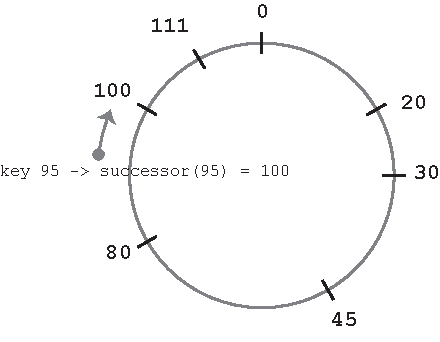
\includegraphics[width=0.5\textwidth]{graphics/chord-ring.pdf}
    \label{fig:chord-ring}}
    \subfloat[Finger table for node 80]{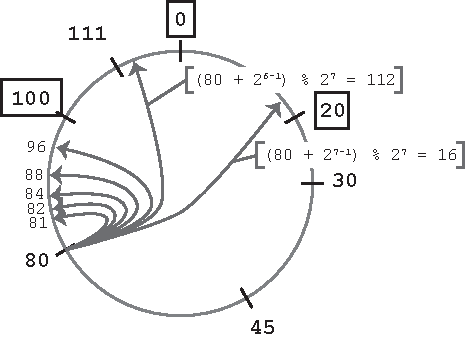
\includegraphics[width=0.5\textwidth]{graphics/chord-finger-table.pdf} \label{fig:chord-finger-table}}
	\caption{Adapted from \cite{chord}}
\label{fig:chord}
\end{figure}

In a very basic implementation of Chord, a peer only needs to know it successor peer. When a key id is queried each peer is passing it to its successor until it reaches the peer, that is responsible of the key space. However, this is not not very efficient because in the worst case a query has to pass the whole circle until it finds its destination. To improve efficiency, Chord introduces a finger table where each peer $\ n $ contains the address of the successor for each entry $\ i $ and $\ (n + 2^{i-1}) \mod 2^m $ where $\ m $ is the size of the circle and $\ 1 \leq i \leq m$. Through the \textit{finger table}, a peer can efficiently route a query request to its destination by using a known peer that is closer to the queried key. \vref{fig:chord-finger-table} shows a sample \textit{finger table} for \textit{Node 80}.
\citet[\S4.3]{chord} describe the process in their paper the following: \say{If $\ n $ can find a node whose ID is closer than its own to $\ k $, that node will know more about the identifier circle in the region of$\ k $ than $\ n $ does. Thus $\ n $ searches its finger table for the node $\ j $ whose ID most immediately precedes $\ k $, and asks $\ j $ for the node it knows whose ID is closest to $\ k $. By repeating this process, $\ n $ learns about nodes with IDs closer and closer to $\ k $}.

\paragraph{Kademlia}\label{par:kademlia}
Kademlia claims to be better than Chord by using a novel \gls{xor} metric which enables them to have a symmetry between keys and node ids \cite[\S1]{kademlia}. They also claim to be better than other algorithms like Pastry in terms of routing, by having one single routing algorithm to locate a peer for a key, while \say{other systems use one algorithm to get
near the target ID and another for the last few hops}\cite[\S1]{kademlia}

The \gls{xor} metric is used to determine a distance from on key to another. As both, the node ids and the keys of the \gls{dht}, are in the same key space this is used to find a node that is closer to the given key. Unlike other distances e.g. euclidian distance it is always unique.
Given the nodes with $\ id = 5 $ in the decimal space, which is  $\ 0101_{b} $ in the binary space, $\ id = 4 = 0100_{b} $ and $\ id = 3 = 0011_{b} $ the euclidean distance $\ d_{euclidean}(5,4) $ and $\ d_{euclidean}(3,4) $ would be the same while the xor distance differs.
\begin{equation}
\begin{aligned}  
    d_ {euclidean} = & | 5-4 | = 1\\
    d_ {euclidean} = & | 3-4 | = 1\\
    d_ {\gls{xor}} = & 0101_{b} \oplus 0100_{b} = 0001_{b} = 1\\
    d_ {\gls{xor}} = & 0011_{b} \oplus 0100_{b} = 0111_{b} = 7\\
  \end{aligned}  
\end{equation}
The \gls{xor} metric is also symmetric $\ d_{\gls{xor}}(a,b) = d_{\gls{xor}}(b,a) $, the distance to itself is zero $\ d_{\gls{xor}}(a,a) = 0 $ and it full fills the triangle inequality $\ d_{\gls{xor}}(a,b) \oplus d_{\gls{xor}}(b,c) = d_{\gls{xor}}(a,c) $ \cite{kademlia}[\S2.1].

By using a binary format for the ids, Kademlia creates a virtual binary tree for each node, where each other node is treated as a leaf node. Thereby the binary tree is divided into subtrees where \say{the highest subtree consists of the half of the binary tree not containing the node. The next subtree consists of the half of the remaining tree not containing the node, and so forth} \cite[\S2]{kademlia}.
\vref{fig:kad-binary-tree} shows a sample binary tree for the black node with the id 0011 with its subtrees that are circled.

\begin{figure}
\centering
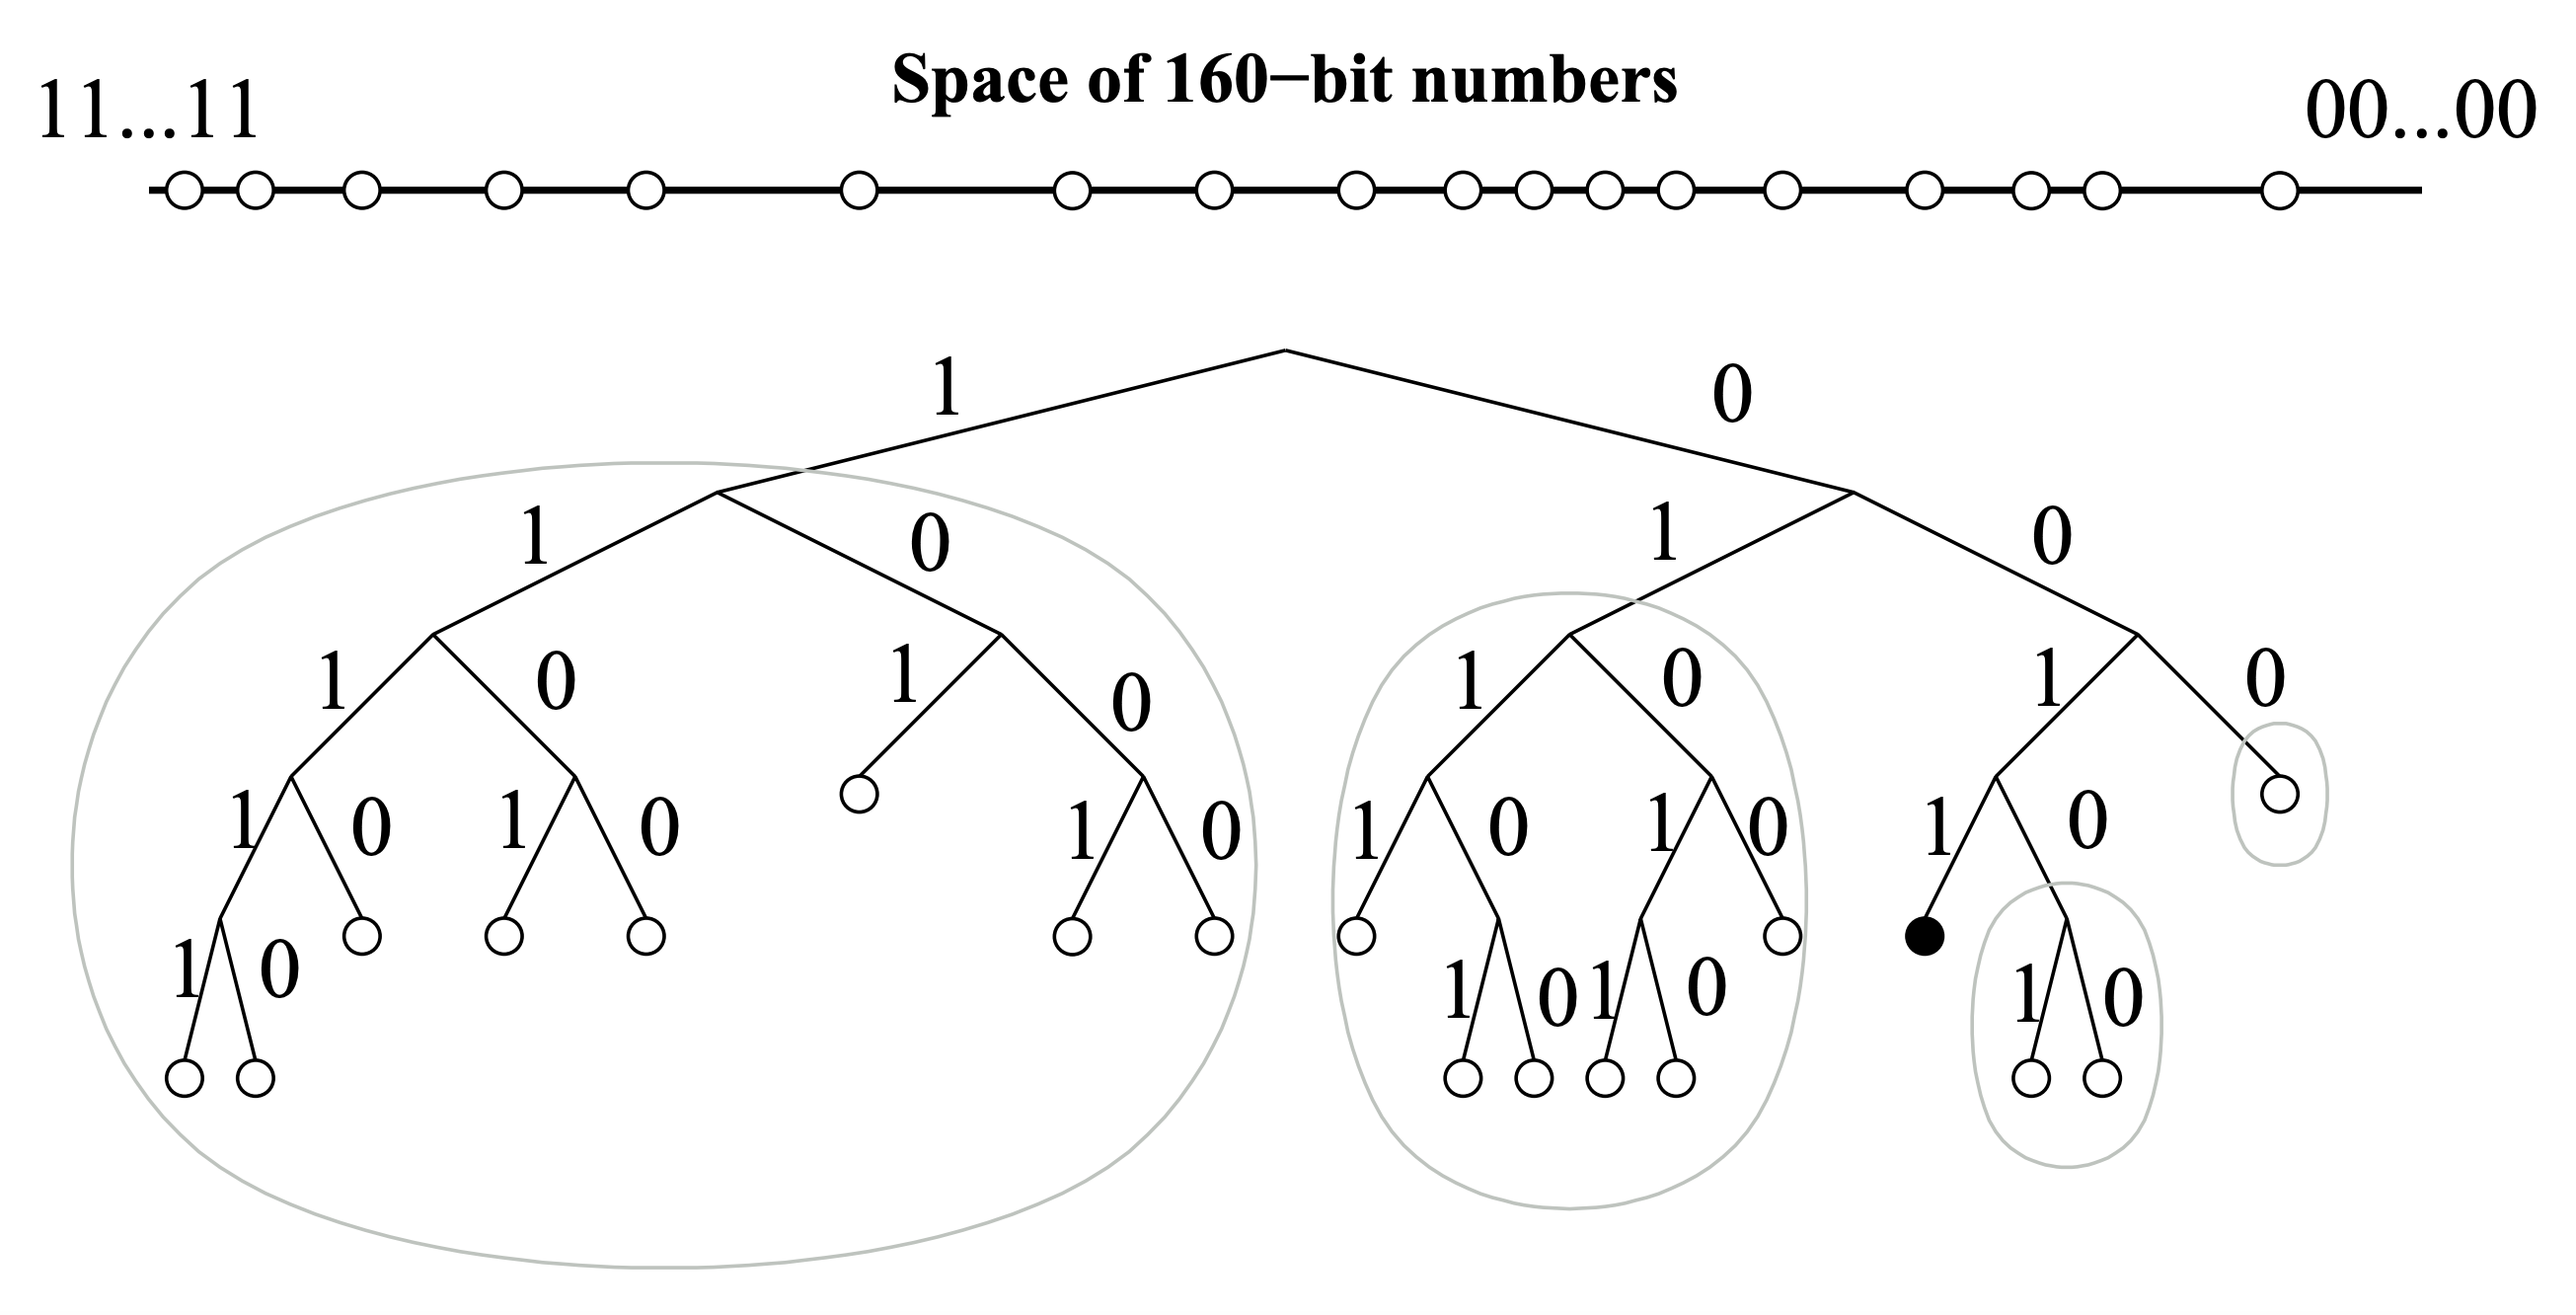
\includegraphics[width=1\textwidth]{graphics/kademlia-binary-tree.png}
\caption{Kademlia binary tree from \cite[\S2]{kademlia}}
\label{fig:kad-binary-tree}
\end{figure}

A node is discovering other nodes over time during message exchanges. Discovered nodes are stored in \say{k-buckets}. Each \say{k-bucket} represents a subtree of the node's virtual binary tree and can have $\ k $ entries. The \say{k-buckets} prevent that the routing table of a node grows to big and also prevents that only close by nodes are stored. By having the $\ k $ limitation, which Kademlia sets to $\ 20 $, maximum 20 discovered node can be stored in each bucket. 
Each entry of the bucket has a \textit{last-seen} property that is updated whenever a message of the node is received. The bucket is sorted by \textit{last-seen}. When a new node is discovered but the bucket is already full Kademlia puts older entries in favour as long as they are alive. To check the liveliness it pings the least recently seen entry in the table. When the node responds, the new discovered node is discarded. However, when the pinged node does not respond, it is removed from the bucket and replaced with the newly discovered node. \citet[\S2.2]{kademlia} argues this with \say{The longer a node has been up, the more likely it is to remain up another hour.}

The design of the protocol ensures that each node knows at least one other node of each subtree and therefore a node can find any other node by its id. To find a \textit{Node X} a \textit{Node A} sends a \textit{FIND\_NODE} request to a node of its buckets that is closest to \textit{Node X}, in terms of the \gls{xor} distance. This \textit{Node B} will then return a \textit{Node C} that is closer to \textit{Node X}. \textit{Node A} will then ask \textit{Node C} for the closest node it knows for \textit{Node X}. This step is repeated until \textit{Node A} finds \textit{Node X}. To speed up the process not only one node is asked but multiple nodes, that are the closest, are asked in parallel. Those nodes also return the closest nodes they know.

Keys are  looked up similar like nodes. A key is stored at a node that is closest to the node id. When a node wants to publish a key it sends a \textit{STORE} request to known nodes that are the closest to the id.
To look up a key, a node sends a \textit{FIND\_VALUE} request to the closest nodes. The process works like finding a node but it terminates as soon as one node returns the stored key.

\subsection{Peer Discovery}
To enter a Peer-to-Peer system there has to be an entry point where new peers can join. 
\citet{p2p-bootstrapping} describe this procedure as \say{P2P bootstrapping}. 
They also give three definitions for the term \say{P2P Bootstrapping}:
\begin{itemize}
        \item Starting a new P2P network (freshly designed protocol)
        \item Once a P2P network is running, any new peer that joins must be integrated into the network
        \item Before a new peer can be integrated into an existing network, the new peer must somehow obtain contact information to at least one node in the existing P2P network
\end{itemize}
\citet[p. 3]{p2p-bootstrapping}

One approach for the boarding process is a central server that provides a list of addresses where a client can enter. In early days of Gnutella a user could enter the network by getting some addresses from a website and pasting them into the Gnutella client \cite[\S3.2]{gnutellaAnalysis}. However, due to Peer Churn it was hard to keep the list of addresses up to date, which resulted in a lot of addresses of peers that were not in the network anymore. In a later version Gnutella tried to solve the problem by providing \say{Gnutella Web Cache} Servers which were maintaining a list of active peers. A client could connect to a \say{Gnutella We Cache} server to obtain a list of active peers to enter the network. Problems that are arising of having a server is, that the server is a single point of failure, may not withstand the traffic (like in the case of Gnutella \cite[\S3.2]{gnutellaAnalysis}) and attackers can obtain lists of active peers which could be attacked then \cite[p. 7]{p2p-bootstrapping}.

Another approach that is taken by BitTorrent is having meta files with a specified entry point. BitTorrent calls those meta files \say{torrents}. The entry point is called \say{tracker}. When a user wants to enter the network it has to obtain a \say{torrent} by visiting one of the various torrent provider websites. Through the torrent file the client is connecting to the tracker and the tracker is making sure to connect the client with other clients to exchange data. BitTorrent has a lot of trackers and anyone can create one by them self. By having multiple instances there is no single point of failure.

libp2p which is used by IPFS has two main boarding mechanisms. One is called \say{mDNS-discovery}. It is used to discover clients in the same network. \say{It emits mDNS beacons to find if there are more peers available. Local area network peers are very useful to peer-to-peer protocols, because of their low latency links.}\cite{ipfs-bootstrapping}.
The second mechanism they have in place is called \say{bootstrap-list}. The \say{bootstrap-list} is a set of addresses a client can connect to. If one fails the client tries the next one. As soon as the client is in the network it stores discovered peer addresses in a local database. The next time the client is using also using those addresses to enter the network.

\subsection{Peer–to–Peer Issues}
Regardless of structure (ring, tree or mesh), \gls{p2p} overlay networks have to overcome similar issues to compete with traditional, client–server paradigms. Because peers naturally have shorter online spans than servers, overlays must be built quickly and constantly adapt to peers joining and leaving. Because peers are part of the infrastructure, such networks must protect against different attack and abuse vectors.

\paragraph{Creation}
- overlay creation -> timetofirstbyte

\paragraph{Maintenance}
- Peer Churn -> unstable network \cite{dht-churn}
For the network to perform well, it is also important to utilise the full potential of all participating devices. As \citet[\S{III}]{multicast-problems} point out, not utilising leaf nodes in a tree network or disregarding a devices individual capabilities, would be two common issues of this category.

\paragraph{Abuse}
- Leechers
- security?

\newpage
\subsection{IPFS}\label{chap:IPFS}

The blockchain movement has sparked new interest in decentralised \gls{p2p} software architectures and networks in academia and the developer community \cite{medium-dnets}. Projects like MaidSafe\footnote{MaidSafe SAFE Network. URL: {https://maidsafe.net}}, Dat\footnote{Dat \gls{p2p} Protocol. URL: {https://datproject.org}} and IPFS\footnote{\label{ipfs}IPFS Protocol. URL: {https://ipfs.io}} are building protocols and \glspl{sdk} for applications and websites with decentralised storage and connectivity. One of these approaches is the self proclaimed \glsfirst{ipfs}. \citet[\S1]{ipfs-whitepaper} sees the current state of the web endangered by rising bandwidth demands, "disappearance of links" and a lack of upgradability. The proposed file system builds upon established distributed communication technologies and could pose an alternative to \gls{http}. It is composed of modular and exchangeable sub–protocols to ensure interoperability and future–proofing. Although \gls{ipfs} does not directly aim to facilitate media streaming, it suggests itself as a viable foundation for any distributed application. The advantage of \gls{ipfs} over similar projects is its clean separation of modules, which are implemented in different programming languages and maintained individually. It has a \gls{js} implementation that works with any modern web browser, instead of requiring proprietary software like MaidSafe's custom browser.

\paragraph{Identity}
To ensure reliable identities and prevent impersonation, each node must be assigned a unique identifier and a private/public key pair. Similar to identity generation in S/Kademlia as described by \citet[\S4.1]{s_kademlia}, \gls{ipfs} requires nodes to solve a pair of crypto puzzles and use a hash of their public key as their identifier. This makes node creation computationally non-trivial and prevents adversaries from flooding the network with nodes \cite[\S3.2]{s_kademlia}.

\paragraph{Network}
\citet[\S3.2]{ipfs-whitepaper} proposes a network stack on top of flexible transport layers such as WebRTC (see \vref{sec:webrtc}) and uTP \cite{utp-micro-torrent-transport-protocol}. Transport reliability, message integrity and authenticity are all defined as optional attributes to be used if the use case requires it. Addresses in \gls{ipfs} are defined in the \lstinline|multiaddr| format which exposes multiple ways to reach a node, be it via proxies, \gls{nat} traversal or though different transport protocols.

\paragraph{Routing}
\gls{ipfs} defines a simple routing interface compliant to that of the Kademlia \gls{dht} (see \vref{par:kademlia}). Peers must be able to find other peers as well as retrieve values from said peers. Values are distinguish by size: up to 1kB is stored directly with peers providing a key and keys to larger values contain a set of seeding peers. \citet[\S3.5]{ipfs-whitepaper} notes "different use cases will call for substantially different routing systems (e.g. DHT in wide network, static HT in local network)". To that end, the routing implementation should be exchangeable.

\paragraph{Data Distribution}
Files in \gls{ipfs} are made up of two abstraction layers. The lower layer consists of blocks of arbitrary binary data. \citet[\S3.4]{ipfs-whitepaper} introduces a BitTorrent inspired protocol called BitSwap. In BitSwap, each node tries to acquire blocks for itself and provide blocks to others. Nodes keep track of how much data others provide and request and punish leechers\footnote{The term leecher has been coined by the BitTorrent community and refers to users who take advantage of the network but do not contribute \cite[\S7.5]{tanenbaum_wetherall_2011}.}. Building upon the block layer, \gls{ipfs} uses a Merkle \gls{dag} to represent files and hierarchies \cite[\S3.5]{ipfs-whitepaper}. All content is addressed by its cryptographic hash \cite{content-centric-networking} and features like deduplication and versioning are built in.

\paragraph{Addressing}
But because files and links are addressed by their hash, modifications have a different hash – or put differently – objects are immutable. To enable persistent addresses for mutable objects, \citet[\S3.7]{ipfs-whitepaper} presents mutable links that can be published under a node's namespace. However, neither nodes nor pieces of content have humanly spellable identifiers and the author presents a workaround using \gls{dns} entries that point to \gls{ipfs} links.

\newpage

\newpage
\section{Video Streaming Applications}

Efficiently delivering streaming video over the internet has long been an active research topic. Non-linearity, rich user interactions and diversification of media sources have driven users from consuming terrestrial television or hard copy video to internet based media platforms.
These platforms and their underlying technologies can be categorised by (1) offered media types and (2) content distribution architecture. Some platforms offer pre-produced videos, be it professional movies or amateur vlogs, to be streamed on demand (\gls{vod}). Other platforms offer live video streams with realtime viewer interactions.
Both type of video offerings can be found to be built upon a centralised or decentralised streaming architecture. \vref{fig:media-platforms-quadrant} shows examples of platforms arranged by category.

\begin{figure}
\centering
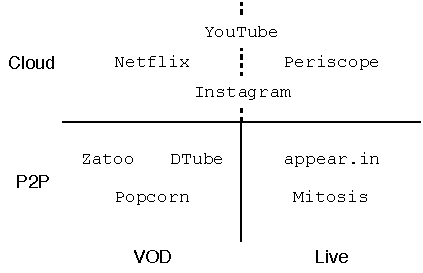
\includegraphics[width=.75\textwidth]{graphics/media-platforms-quadrant.pdf}
\caption{Examples of media platforms by delivery and content category}
\label{fig:media-platforms-quadrant}
\end{figure}

\subsection{Centralised Streaming}

The most popular video platforms, YouTube\footnote{Youtube. URL: {https://www.youtube.com}} and Netflix\footnote{Netflix. URL: {https://www.netflix.com}}, currently account for TODO percent of internet traffic \cite[p 18]{phenomena-report}. Dealing with such extreme user numbers, centralised video delivery architectures are complex and costly \cite{market-driven-p2p}. To deliver compelling \gls{qos} to users, platforms must ensure their networks can retrieve content from a live source or their catalogue with low latency and deliver it in a format optimal for the end users' device and network capabilities. There must be a global server infrastructure for storing, caching and delivering content. Platforms that allow user-generated content must also provide ingress servers, that accept video uploads from users.

These expenses drive platform providers to heavy use of video advertising or subscription models.

\paragraph{Ingress}
Platforms with user-generated content have grown in popularity and significance and, according to \citet{twitch-case}, can be characterised by opening content creation to all of their users and allowing video consumers to give realtime feedback in the form of chats or likes. This interactivity poses tight constraints on latency, or users can become frustrated \cite{TODO}. Periscope, for example, constraints its chat function to the first 100-200 viewers per stream \cite{TODO}. These early participants will be provided with a low latency \gls{rtmp} video stream \cite{TODO}. Subsequent viewers will be served an \gls{hls} video from a global \gls{cdn}. The latter introduces two further sources of delay \cite[\S2-3{periscope-experience}: 1) \gls{hls} segments the video into smaller files, so the duration of such a chunk adds to overall latency. 2) According to network analysis by \citet{periscope-experience} Periscope uses different \textit{Cloud Computing} providers for ingress and \gls{cdn} use.

Twitch, for example, reserves computationally expensive trans-coding of live streams for its premium users \cite[\S2]{twitch-study}. That means, viewers of free channels can only receive the video in the format it was originally uploaded in. Since, unlike Periscope, Twitch also offers access to streams through their website \cite{TODO}, this excludes users from content in formats incompatible with their browser. If a channel subscribes to their premium service trans-coding introduces a delay of up to 10 seconds \cite[\S4.2]{twitch-study}.

\citet[III A.]{content-harvest-network} argue, that the so-called \textit{first mile} between the live video producer and the systems ingress server bears a significant optimisation opportunity. Because upload may be hindered by unstable network conditions, any delay directly impacts the \gls{qoe} of all viewers of the stream.

\paragraph{Transcoding}
SFU or whatevs, Transcoding units

\paragraph{Quality of Experience}
\citet*{personalized-live-streaming-experience} propose schemes to optimise variable video bitrates to improve the perceived \gls{goe} for viewers.

\paragraph{Delivery}
Because HTTP streaming protocols are not built for multicasting, even popular live streams, that many users view simultaneously, have to be delivered to each device individually. Therefore, providers use multiple server farms \cite{TODO-network-book} in strategic geographic locations of their user market. Streams must be routed intelligently from ingress to egress locations within a provider's network. Predicting a streams popularity and allocating resources in locations geographically close to viewer demand can help reduce latency \cite{TODO}.

According to \citet{TODO}, the strategy of Twitch is to serve content from the vicinity of every \gls{ipx}. Social photo and video sharing site Instagram, on the other hand, goes even further and serves content from locations in most major cities of its user market \cite{TODO}. These efforts to bringing server resources as close to users as possible are often referred to as edge or fog computing \cite{fog-computing, object-store-fog-edge-ipfs}.

Despite all efforts, especially less financially secured platforms struggle to come up with enough resources to deliver \gls{qos} without compromise.
...

- Cisco says mobile video streaming is lit

\paragraph{Social Aspects}
censorship vs piracy

\begin{figure}
\centering
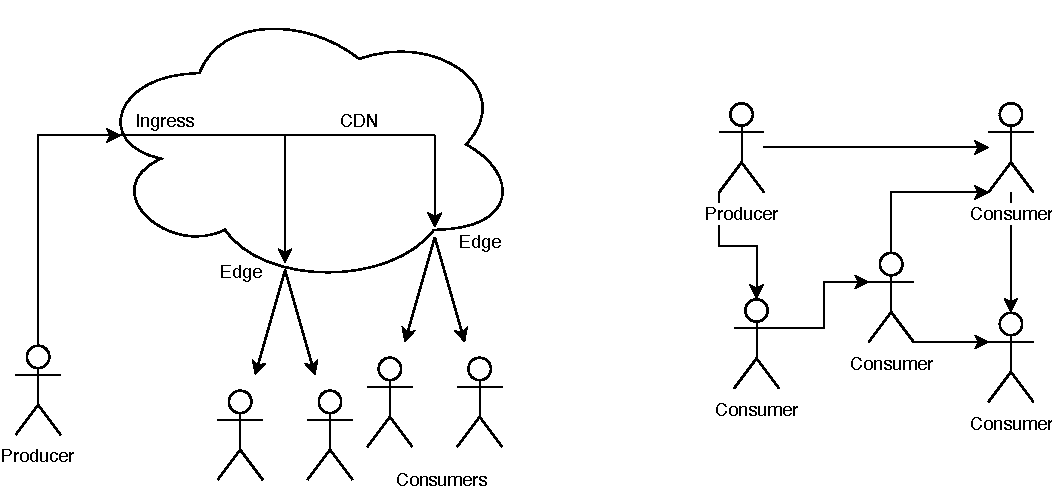
\includegraphics[width=.5\textwidth]{graphics/streaming-types.pdf}
\caption{Centralised versus decentralised video streaming architecture}
\label{fig:pipeline}
\end{figure}

\subsection{Decentralised Streaming}

In contrast, decentralised video streaming technologies build multicast streaming on top of an overlay network in the application space. These overlays can be categorised as tree or mesh shaped or a combination thereof. Each peer becomes part of the network and has to assist in its maintenance and content delivery. Decentralised streaming approaches need to handle peers joining and leaving the network, called \textit{peer churn} \cite[\S7.5]{tanenbaum_wetherall_2011}. Like centralised platforms, they must also cope with varying network performance of its users. However, upload capacity becomes a important factor for every peer, not just content producing ones. This means, that finding a compromise between the depth of the tree or mesh structure and the amount of outward connections each node has to maintain is crucial for the system's performance \cite[\SIII.A]{multicast-problems}.

\paragraph{Content Discovery}
In fully decentralised approaches, content discovery is another issue to consider. Whereas centralised media platforms can index, aggregate and even recommend content to users by consulting their databases, decentralised applications lack such central look–up tables by design. Information about peer and content availability must be propagated through the network, creating further traffic and computational overhead.

\paragraph{DONet}
DONet, which was first implemented in the widely researched CoolStreaming, was introduced by \citet{coolstreaming}. It constructs a mesh of peers gossiping (\ref{gossiping}) about available content, members of the network and direct connections. Each peer maintains an incomplete view of the network and a set of peer partnerships. Video streams are split into segments of a defined length and the segments are broadcasted through the network individually. Nodes request segments from their partners, cache segments they receive and add them to their own playback buffer \cite[\SIII.B]{coolstreaming}. When a node detects a stalling upstream partner, it tries to find a better source \cite[\SIV.A]{coolstreaming-design-theory}.

\paragraph{AnySee}
Mesh–based streaming networks like CoolStreaming can achieve good utilisation of peer bandwidth and discover fresh peers with low overhead \cite[\SII]{anysee}. However, \citet[\SIII]{anysee} find that, "Due to the random selection algorithm, the quality of service cannot be guaranteed, such as the startup delay". AnySee evolves \gls{p2p} streaming nodes with a set of manager components \citep[\SIII.B-F]{anysee}. 1) The \textit{Mesh-based Overlay Manager} actively tries to align the mesh network with the physical network by flooding its neighbourhood with \gls{ttl}–bound messages and re–aligning overlay connections. 2) The \textit{Single Overlay Manager} measures and propagates a nodes time offset from the video source and ensures the streaming path is arranged according to this offset. 3) The \textit{Inter-overlay Optimization Manager} secures a set of backup streaming paths through a delay–based tracing algorithm. 4) The \textit{Key Node Manager} queues requests and prioritises stream requests from other peers. 5) The \textit{Buffer Manager}'s task is to request upstream video and providing it to the applications \gls{ui}.

+ continuouity index
+ buffer size 120 vs 40 seconds
- timestamps be shitty

Further, AnySee introduces location awareness to encourage peer partnering close to their geographical vicinity \citep[\SV.B.1]{anysee}. In their initial implementation, this was achieved by matching \gls{ip} addresses of their research network (\gls{cernet}) to known building locations.

\paragraph{HLPSP}
Another refinement to CoolStreaming was introduced by \citet*{hlpsp} called \gls{hlpsp}. This approach creates a layered hierarchy in which peers with higher uploads are positioned in levels closer to the video source. Peers then serve other peers in their own or subsequent levels \cite[\S3]{hlpsp}. The gauging of bandwidth is left up to the network entry point (also referred to as signal server or tracker). This central server assigns a level to a newcomer and provides a list of possible connection partners. If not enough suitable partners are found, the tracker scans the hierarchy and downgrades peers to free capacity on the newcomers level \cite[\S3.3.2]{hlpsp}. This results in efficient bandwidth utilisation, but only accounts for single source scenarios.

- routing
- overlay creation -> timetofirstbyte
- ...problems of streamer cite

\newpage

\chapter{Introduction}

\chapter{Analysis}
- Simulation
- Hard limits
- Discussion

\section{Future Work}
- Persistence via IPFS
- End-To-End Encryption of the data-layer
- Crypto puzzle (proof of work) to enter system / send messages (spam prevention) 
%
%
%\renewcommand{\appendixtocname}{Anhang}
%\renewcommand{\appendixname}{Anhang}
%\renewcommand{\appendixpagename}{Anhang}
\appendix

\clearpage

%\printindex

\printbibliography

\ifdeutsch
Alle URLs wurden zuletzt am 10.\,03.\,2019 geprüft.
\else
All links were last followed on March 10, 2019.
\fi

\pagestyle{empty}
\renewcommand*{\chapterpagestyle}{empty}
\Versicherung
\end{document}
